\documentclass[12pt, a4paper, onecolumn, oneside, final]{report}
\usepackage[latin1]{inputenc}
\usepackage[bahasa]{babel}
\usepackage{amsmath}
\usepackage{amsfonts}
\usepackage{amssymb}
\usepackage{tocloft}
\usepackage[left= 3.5cm,right=3cm,top=3cm,bottom=3cm]{geometry}
\usepackage{indentfirst}
\usepackage{amsmath,amssymb,amsfonts,amsthm}
\usepackage{array}
\usepackage{caption}
\usepackage{wrapfig}
\usepackage{graphicx}
\usepackage{varwidth}
\usepackage{float}
\usepackage{indentfirst}
\usepackage{textcomp}
\usepackage{lmodern}
\usepackage{enumerate}
\usepackage{tabularx}
\usepackage{microtype}
%\usepackage[framed]{matlab-prettifier}
\usepackage{inputenc}
\usepackage{tikz}
\usepackage{xcolor,colortbl}
\usepackage{multirow}
\usepackage{times}
\usepackage{float}
\usepackage{hyperref}
\hypersetup{colorlinks=true,
	linkcolor=black,
	filecolor=black,      
	urlcolor=blue,}
%	pdfpagemode=FullScreen,}
\urlstyle{same}
\usepackage{setspace}
\usepackage{apacite}
\usepackage{enumitem}
\usepackage[labelsep=period]{caption}
%\usepackage{pbsi}
\usepackage[T1]{fontenc}
\usepackage{esint}
\usepackage{lipsum}
\usepackage{multirow}
\usepackage{ragged2e}
\usepackage[justification=centering]{caption}
%%
% Hyphenation untuk Indonesia
%
% @author  Andreas Febrian
% @version 2.02
% @edit by Ichlasul Affan
%
% Tambahkan cara pemenggalan kata-kata yang salah dipenggal secara otomatis
% oleh LaTeX. Jika kata tersebut dapat dipenggal dengan benar, maka tidak
% perlu ditambahkan dalam berkas ini. Tanda pemenggalan kata menggunakan
% tanda '-'; contoh:
% menarik
%   --> pemenggalan: me-na-rik
%


% Silakan ganti ke bahasa Inggris (\selectlanguage{english}) jika Anda merasa terlalu banyak kata bahasa Inggris yang pemenggalannya tidak benar.
\selectlanguage{bahasa}


\hyphenation{
    % alphabhet A
    a-na-li-sa a-tur
    a-pli-ka-si
    % alphabhet B
    ba-ngun-an
    be-be-ra-pa
    ber-ge-rak
    ber-ke-lan-jut-an
    ber-pe-nga-ruh
    % alphabhet C
    ca-ri
    % alphabhet D
    di-da-pat-kan di-sim-pan di-pim-pin de-ngan da-e-rah di-ba-ngun da-pat di-nya-ta-kan
    di-sim-bol-kan di-pi-lih di-li-hat de-fi-ni-si di-de-fi-ni-si-kan di-mi-li-ki
    % alphabhet E
    e-ner-gi eks-klu-sif
    % alphabhet F
    fa-si-li-tas
    % alphabhet G
    ga-bung-an ge-rak
    % alphabhet H
    ha-lang-an
    % alphabhet I
    % alphabhet J
    % alphabhet K
    ke-hi-lang-an
    ku-ning
    kua-li-tas ka-me-ra ke-mung-kin-an ke-se-pa-ham-an
    % alphabhet L
    ling-kung-an
    % alphabhet M
    me-neng-ah
    meng-a-tas-i me-mung-kin-kan me-nge-na-i me-ngi-rim-kan
    meng-u-bah meng-a-dap-ta-si me-nya-ta-kan mo-di-fi-ka-si
    meng-a-tur meng-a-rah-kan mi-lik
    % alphabhet N
    nya-ta non-eks-klu-sif
    % alphabhet O
    % alphabhet P
	pe-nye-rap-an
	pe-ngon-trol
    pe-mo-del-an
    pe-ran  pe-ran-an-nya
    pem-ba-ngun-an pre-si-den pe-me-rin-tah prio-ri-tas peng-am-bil-an
    peng-ga-bung-an pe-nga-was-an pe-ngem-bang-an
    pe-nga-ruh pa-ra-lel-is-me per-hi-tung-an per-ma-sa-lah-an
    pen-ca-ri-an pen-ce-ta-kan peng-struk-tur-an pen-ting pen-ting-nya
    % alphabhet Q
    % alphabhet R
    ran-cang-an
    % alphabhet S
    si-mu-la-si sa-ngat
    % alphabhet T
    te-ngah
    ter-da-pat
    trans-for-ma-si
    % alphabhet U
    % alphabhet V
    va-ri-an va-ri-a-si
    % alphabhet W
    % alphabhet X
    % alphabhet Y
    % alphabhet Z
    % special
}

\usepackage{amsmath,amssymb,amsfonts,amsthm}
\renewcommand{\chaptername}{BAB}
%\usepackage{setspace}

\setcounter{tocdepth}{1}

\definecolor{green}{rgb}{0.1,0.1,0.1}
\newcommand{\done}{\cellcolor{teal}done}  %{0.9}
\newcommand{\hcyan}[1]{{\color{teal} #1}}

\newtheorem{theorem}{Dalil}
\newtheorem{corollary}{Akibat}
\newtheorem{lemma}{Lemma}
\newcommand\at[2]{\left.#1\right|_{#2}}
\theoremstyle{definition}
\newtheorem{definition}{Definisi}{}
\newtheorem{example}{\textsf{Contoh}}

\newenvironment{bukti}[1][Bukti]{\noindent{\it\textit{#1. }}}
{\hspace{\stretch{1}}\rule{.5em}{.5em}}

\DeclareMathOperator{\mo}{mod\,}
\DeclareMathOperator{\ord}{ord}
\DeclareMathOperator{\fpb}{fpb}
\newcommand{\defi}{\overset{\mbox{\tiny{\sf def}}}{=}}
\newcommand{\znz}{\Bbb Z/n\Bbb Z}\newcommand{\zpz}{\Bbb Z/p\Bbb Z}
\numberwithin{equation}{chapter}

\setcounter{tocdepth}{3}
\setcounter{secnumdepth}{3}

\setlength\parindent{12.5mm}

\usepackage{blindtext}
\renewcommand\cftbeforetoctitleskip{-1cm}
 \renewcommand\cftbeforeloftitleskip{-1cm}
 \renewcommand\cftbeforelottitleskip{-1cm}
\renewcommand{\cftdotsep}{1}
\renewcommand{\cftchapleader}{\cftdotfill{\cftsecdotsep}}

\renewcommand{\contentsname}{DAFTAR ISI}
\renewcommand{\cfttoctitlefont}{\hfil\Large\bfseries\MakeUppercase}
\renewcommand{\cftchapfont}{\bfseries}
\renewcommand{\cftchappagefont}{\bfseries}
\renewcommand{\cftchappresnum}{BAB }
\renewcommand{\cftchapnumwidth}{3.7em}

\renewcommand{\cftlottitlefont}{\hfil\large\bfseries\MakeUppercase}
\renewcommand{\cfttabpresnum}{Tabel }
\renewcommand{\cfttabnumwidth}{6em}

\renewcommand{\cftloftitlefont}{\hfil\large\bfseries\MakeUppercase}
\renewcommand{\cftfigpresnum}{Gambar }
\renewcommand{\cftfignumwidth}{6em}
\renewcommand{\figurename}{Gambar}

\makeatletter
\def\ps@myPS{%
    \def\@oddfoot{\null\hfill\thepage}
    \def\@evenfoot{\thepage}%
    \def\@evenhead{\null\hfil\slshape\leftmark}%
    \def\@oddhead{{\slshape\rightmark}}}%
\makeatother

\makeatletter % default is "\newcommand\@chapapp{\chaptername}"
\renewcommand\@chapapp{\textls[40]{\MakeUppercase{\chaptername}}}
\makeatletter

\usepackage{titlesec}
% 1. Judul bab ditengah
\titleformat{\chapter}[display]
 {\normalfont\large\bfseries\centering}
 {\chaptertitlename\ \Roman{chapter}}{0pt}{\large}
% 2. Font section 12pt dan tambah titik section, so 1.1 menjadi 1.1.
\titlespacing{\chapter}{0pt}{50pt}{\baselineskip}
\titleformat{\section}[block] %tambah block untuk menampilkan format angka 
 {\normalfont\fontsize{12}{15}\bfseries}{\thesection.}{1em}{}
% 3. Font subsection 12pt dan tambah titik subsection
 \titleformat{\subsection}[block] %tambah block untuk menampilkan format angka 
 {\normalfont\fontsize{12}{15}\bfseries}{\thesubsection.}{1em}{} 
% 4. Hapus spasi setelah bab
\makeatletter
\def\ttl@mkchap@i#1#2#3#4#5#6#7{%
 \ttl@assign\@tempskipa#3\relax\beforetitleunit
 \vspace{\@tempskipa}%<<<<<< REMOVE THE * AFTER \vspace
 \global\@afterindenttrue
 \ifcase#5 \global\@afterindentfalse\fi
 \ttl@assign\@tempskipb#4\relax\aftertitleunit
 \ttl@topmode{\@tempskipb}{%
 \ttl@select{#6}{#1}{#2}{#7}}%
 \ttl@finmarks % Outside the box!
 \@ifundefined{ttlp@#6}{}{\ttlp@write{#6}}}
 
 \usetikzlibrary{shapes.geometric, arrows}
%Spasi sebelum dan sesudah judul sub bab
%\titlespacing*{\section}
%{0pt}{5.5ex plus 1ex minus .2ex}{4.3ex plus .2ex}
%\titlespacing*{\subsection}
%{0pt}{5.5ex plus 1ex minus .2ex}{4.3ex plus .2ex}

\newcommand{\listappendicesname}{DAFTAR LAMPIRAN}
\newlistof{appendices}{apc}{\listappendicesname}
\newcommand{\appendices}[1]{\addcontentsline{apc}{appendices}{#1}}
\renewcommand\cftbeforeapctitleskip{-1cm}
\renewcommand{\cftapctitlefont}{\hfil\large\bfseries\MakeUppercase}

\newcommand{\newappendix}[1]{\section*{#1}\appendices{#1}}

% Tambah kata ejaan yang salah di Latex 
\hyphenation{
    alphabhet A 
    alphabhet B 
    alphabhet C 
    alphabhet D 
    alphabhet E
    alphabhet F 
    alphabhet G 
    alphabhet H 
    alphabhet I
    alphabhet J
    alphabhet K 
    alphabhet L
    alphabhet M 
    alphabhet N 
    alphabhet O
    alphabhet P 
    alphabhet Q
    alphabhet R
    alphabhet S 
    alphabhet T 
    alphabhet U
    alphabhet V
    alphabhet W 
    alphabhet X
    alphabhet Y
    alphabhet Z
    special}
  \makeatletter
\renewcommand*\@pnumwidth{3em}
\makeatother

%=====================================================================
\begin{document}

\tikzstyle{rect} = [draw, rectangle, fill=white!20, text width=25em, text centered, minimum height=2em]%text width=20em/13em
\tikzstyle{elli} = [draw, ellipse, fill=white!20, minimum height=2em]
\tikzstyle{circ} = [draw, circle, fill=white!20, minimum height=2em, inner sep=10pt]
\tikzstyle{diam} = [draw, diamond, fill=white!20, text width=6em, text badly centered, inner sep=0pt]
\tikzstyle{line} = [draw, -latex']
%=====================================================================
\pagenumbering{roman}
%=====================================================================
% Halaman Judul
%\addtocontents{toc}{~\hfill{\it Halaman}\par}
\addtocontents{toc}{\begingroup\protect\setlength{\protect\cftsecindent}{-\leftmargin}}
%\addcontentsline{toc}{section}{\protect\numberline{}Judul}
\addtocontents{toc}{\endgroup}
\begin{spacing}{1}
	\begin{center}
		{\Large\textbf{APLIKASI MODEL NUMERIK TIGA DIMENSI UNTUK SIMULASI HIDRODINAMIKA LAUT}}\\[1.0cm]
	\end{center}
	\vspace*{0.8cm} 
	
	\begin{center}
		
		% harus dalam 16pt Times New Roman
		\large{\textbf{PROPOSAL DISERTASI}}
		\\\vspace*{1.8cm}    
		\normalsize{Diajukan untuk melengkapi tugas-tugas dan \\
			memenuhi syarat-syarat guna pelaksanaan penelitian Disertasi}\\[1.5cm]
		%\vspace*{0.3 cm}    
		%% harus dalam 16pt Times New Roman
		\vspace*{1cm}  
		{\large Oleh:}\\
		\vspace*{1cm}       
		% penulis dan NIM
		\large{\textbf{\underline{MUH. NUR HIDAYAT}}}
		\\\large{\textbf{2108201010005}} 
	\end{center}\vspace*{1cm}   
	
	\begin{figure}[h]
		\centering
		
\includegraphics[width=4cm]{contents/USK} %logo universitas
	\end{figure}
	\vspace*{1.5cm}   
	
	\begin{center}
		% informasi mengenai fakultas dan program studi
		\textbf{PROGRAM STUDI DOKTOR MATEMATIKA DAN APLIKASI SAINS\\
			PROGRAM PASCASARJANA \\
			UNIVERSITAS SYIAH KUALA\\
			DARUSSALAM, BANDA ACEH\\
			JUNI, 2023}
	\end{center}
	\thispagestyle{empty}
\end{spacing}
%=====================================================================
% Halaman Pengesahan
\pagebreak
\chapter*{PENGESAHAN}
\addtocontents{toc}{\begingroup\protect\setlength{\protect\cftsecindent}{-\leftmargin}}
%\addcontentsline{toc}{section}{\protect\numberline{}Pengesahan}	
\addtocontents{toc}{\endgroup}
\setcounter{page}{2}
\vspace{1.5pc}

\begin{center}
	\normalsize
	\noindent
	\begin{tabular}{l l l}
		Judul Disertasi \verb"  " &: Aplikasi Model Numerik Tiga Dimensi untuk Simulasi \\
		& \; Hidrodinamika Laut \\
		Nama Mahasiswa &: Muh. Nur Hidayat \\
		NPM &: 2209300070026 \\
		Program Studi	&: Doktor Matematika dan Aplikasi Sains\\ 
	\end{tabular} \\
\end{center}

\begin{center}
	\vspace{3cm}
	Menyetujui\\
	Komisi Pembimbing, \\
	Promotor \\
	\vspace{2cm}
	\underline{Prof. Dr. Ir. Syamsul Rizal} \\
	NIP. 196101221987031003
	\vspace{1cm}
	
	\begin{tabular}{l l }
		Ko-Promotor I,\verb"                       " & Ko-Promotor II, \verb"            "\\[2.25cm]
		\underline{Prof. Dr. Marwan Ramli, S.Si.,M.Si.} & \underline{Prof. Dr. Muchlisin Z.A, S.Pi.,M.Sc.}\\
		NIP. 197111251999031003 & NIP. 197109111999031003
	\end{tabular}
\end{center}

\begin{center}
	\vspace{0.5cm}
	Mengetahui\\%[0.5cm]
	
	\vspace{1cm}
	
	\begin{tabular}{l l }
		Ketua Program Studi\verb"                  " & \verb" "Direktur Program Pascasarjana\\
		Doktor Matematika dan Aplikasi Sains, & \verb" "Universitas Syiah Kuala,\\[2.25cm]
		\underline{Prof. Dr.rer.nat. Rinaldi Idroes, S.Si.} & \verb" "\underline{Prof. Dr. Ir. Darusman, M.Sc.}\\
		NIP. 196808251994031003 & \verb" "NIP. 196210091987021001
	\end{tabular}
\end{center}
%\vspace{0.3cm}
%\begin{center}
%	
%\end{center}
%\thispagestyle{empty}

%\input{LPS}
%=====================================================================
% Halaman Bebas Plagiasi
%\pagebreak
%\chapter*{PERNYATAAN BEBAS PLAGIASI}
%\addtocontents{toc}{\begingroup\protect\setlength{\protect\cftsecindent}{-\leftmargin}}
%\addcontentsline{toc}{section}{\protect\numberline{}Pernyataan Bebas Plagiasi}	
%\addtocontents{toc}{\endgroup}
%\begin{spacing}{1.5}
	\pagestyle{empty}
	\begin{center}
		\vskip 1cm
		\lipsum[1-3]
	\end{center}
\end{spacing}
\pagestyle{empty}
%=====================================================================
% Halaman Abstrak
%\pagebreak
%\chapter*{ABSTRAK}
%\addtocontents{toc}{\begingroup\protect\setlength{\protect\cftsecindent}{-\leftmargin}}
%%\addcontentsline{toc}{section}{\protect\numberline{}Abstrak}	
%\addtocontents{toc}{\endgroup}
%\begin{spacing}{1.5}
	\pagestyle{empty}
	\begin{center}
		\vskip 1cm
		\lipsum[1-2]
	\end{center}
\end{spacing}
\pagestyle{empty}
%=====================================================================
% Halaman Kata Pengantar
\pagebreak
\chapter*{KATA PENGANTAR}	
\addtocontents{toc}{\begingroup\protect\setlength{\protect\cftsecindent}{-\leftmargin}}
\addcontentsline{toc}{section}{\protect\numberline{}\textbf{KATA PENGANTAR}}
\addtocontents{toc}{\endgroup}
\begin{spacing}{1.5}
	\pagestyle{empty}
	
	\vskip 1cm
	\par Puji syukur kehadirat Allah SWT yang telah melimpahkan nikmat karunia-Nya sehingga proposal penelitian yang berjudul \textbf{Aplikasi Model Numerik Tiga Dimensi untuk Simulasi Hidrodinamika Laut} dapat terselesaikan dengan baik. Penelitian ini dilakukan untuk memenuhi salah satu syarat dalam memperoleh gelar Doktor pada Program Studi Doktor Matematika dan Aplikasi Sains, Universitas Syiah Kuala.
	\par Penyusunan proposal penelitian ini tidak dapat selesai tanpa bantuan dari tim pembimbing. Oleh karena itu, ucapan terima  kasih disampaikan kepada pihak-pihak tersebut.
	\par Proposal penelitian ini tidak luput dari segala kekurangan, baik dalam hal penulisan maupun pembahasan dari topik penelitian. Oleh sebab itu, diperlukan saran demi penyusunan penelitian yang lebih baik. Semoga penelitian dapat memberi manfaat bagi pembaca untuk melaksanakan penelitian selanjutnya.
	\vskip 1cm  
	\begin{flushright}
		Banda Aceh, 15 Juni 2023
		\vskip 2cm
		Penulis	
	\end{flushright}
\end{spacing}
\pagestyle{empty}
%=====================================================================
% Halaman Ringkasan
\pagebreak
\chapter*{RINGKASAN}
\addtocontents{toc}{\begingroup\protect\setlength{\protect\cftsecindent}{-\leftmargin}}
\addcontentsline{toc}{section}{\protect\numberline{}\textbf{RINGKASAN}}	
\addtocontents{toc}{\endgroup}
\begin{spacing}{1.5}
	\pagestyle{empty}
	\begin{center}
		\vskip 1cm
		\justifying
		Samudera Hindia adalah samudera terbesar ketiga di dunia, meliputi sekitar 19.8\% dari total volume lautan dan merupakan lautan yang sangat berpengaruh bagi ekosistem di Bumi. Cakupan wilayah dari Samudera Hindia termasuk di dalamnya Teluk Benggala (\textit{Bay of Bengal} (BoB)), Laut Andaman, Selat Malaka, dan Perairan Aceh. Dengan cakupan wilayah yang begitu luas, Samudera Hindia merupakan penyumbang besar bagi sistem iklim dunia dan oleh karena itu sangat penting untuk dapat diprediksi. Pengembangan model kelautan berusaha untuk menggambarkan iklim global dengan cukup baik disertai dengan pengamatan. Namun, variabilitas spasial dan temporal perlu dipahami untuk prediksi yang lebih baik. Kajian mengenai kontribusi parameter meteorologi: \textit{2m air temperature, 2m specific humidity, convective precipitation rate, sea level pressure, wind stress U}, dan \textit{wind stress V} terhadap variabilitas MLD menggunakan data output model resolusi tinggi untuk jangka panjang belum pernah dilakukan sebelumnya khususnya untuk wilayah perairan Aceh, oleh karena itu penelitian ini bertujuan untuk menginvestigasi MLD berdasarkan parameter meteorologi yang telah disebutkan sebelumnya. Analisis dengan model iklim ditekankan sebagai verifikasi untuk observasi MLD yang dilakukan pada sampel stasiun wilayah peneltian. Pada akhirnya, dari hasil analisis yang dilakukan akan diperoleh hubungan antara parameter meteorologi dan MLD. Penelitian ini diharapkan mampu memberikan kontribusi ilmiah dan memperkaya pengetahuan tentang kedalaman lapisan campuran. Hal ini karena kedalaman lapisan campuran berperan penting secara iklim fisik dalam hal menentukan interval kisaran temperatur di wilayah laut dan pesisir. Sebagai tambahan, panas yang tersimpan dalam lapisan campuran menyediakan sumber panas yang mendorong variabilitas global seperti El Ni$\tilde{n}$o. Kedalaman lapisan campuran juga berperan dalam menentukan tingkatan rata-rata cahaya yang dapat dilihat oleh organisme laut seperti fitoplankton. Selain itu, dari periodesitas model iklim yang diperoleh akan bermanfaat untuk tujuan fishing ground, mitigasi perubahan iklim dan bencana hidro-oseanografi, tata ruang dan konservasi laut, dan sumber energi terbarukan.
	\end{center}
\end{spacing}
\pagestyle{empty}
%=====================================================================
% Halaman Daftar Isi
\pagebreak
\addtocontents{toc}{\begingroup\protect\setlength{\protect\cftsecindent}{-\leftmargin}}
\addcontentsline{toc}{section}{\protect\numberline{}\textbf{DAFTAR ISI}}	
\addtocontents{toc}{\endgroup}{
\hypersetup{linkcolor=black}
\tableofcontents}
%=====================================================================
% Halaman Daftar Tabel
\pagebreak
\renewcommand{\listtablename}{DAFTAR TABEL}
\addtocontents{toc}{\begingroup\protect\setlength{\protect\cftsecindent}{-\leftmargin}}
\addcontentsline{toc}{section}{\protect\numberline{}\textbf{DAFTAR TABEL}}	
\addtocontents{toc}{\endgroup}
%\addtocontents{lot}{~\hfill{\it Halaman}\par}
{\hypersetup{linkcolor=black}
\listoftables}
%=====================================================================
% Halaman Daftar Gambar
\pagebreak
\renewcommand{\listfigurename}{DAFTAR GAMBAR}
%\addtocontents{lof}{~\hfill{\it Halaman}\par}
\addtocontents{toc}{\begingroup\protect\setlength{\protect\cftsecindent}{-\leftmargin}}
\addcontentsline{toc}{section}{\protect\numberline{}\textbf{DAFTAR GAMBAR}}	
\addtocontents{toc}{\endgroup}
{\hypersetup{linkcolor=black}
\listoffigures}
%=====================================================================
% Halaman Daftar Simbol
%\pagebreak
%\chapter*{DAFTAR SIMBOL}
%\addtocontents{toc}{\begingroup\protect\setlength{\protect\cftsecindent}{-\leftmargin}}
%\addcontentsline{toc}{section}{\protect\numberline{}\textbf{DAFTAR SIMBOL}}	
%\addtocontents{toc}{\endgroup}
%\vspace{1.5pc}
\vspace{1.5pc}
\begin{center}
\begin{tabular}{lp{0.75\textwidth}}

\end{tabular}
\end{center}
%=====================================================================
% Halaman Daftar Lampiran
%\pagebreak 
%{\hypersetup{linkcolor=black}
%\listofappendices}
%%\addtocontents{apc}{~\hfill{\it Halaman}\par}
%\addtocontents{toc}{\begingroup\protect\setlength{\protect\cftsecindent}{-\leftmargin}}
%\addcontentsline{toc}{section}{\protect\numberline{}\textbf{DAFTAR LAMPIRAN}}	
%\addtocontents{toc}{\endgroup}
%=====================================================================
% Halaman Persembahan
%\pagebreak
%\chapter*{PERSEMBAHAN}
%\addtocontents{toc}{\begingroup\protect\setlength{\protect\cftsecindent}{-\leftmargin}}
%\addcontentsline{toc}{section}{\protect\numberline{}PERSEMBAHAN}	
%\addtocontents{toc}{\endgroup}
%\begin{spacing}{1.5}
	\pagestyle{empty}
	\begin{center}
		\vskip 1cm
		\lipsum[1-3]
	\end{center}
\end{spacing}
\pagestyle{empty}
%=====================================================================
\newpage
\makeatother
\newpagestyle{chapterpage}{\setfoot{}{}{\thepage}}
\assignpagestyle\chapter{chapterpage}
\setcounter{page}{1}
\pagenumbering{arabic}
\pagestyle{myPS}
\def\thechapter{\Roman{chapter}} 
\def\thesection{\arabic{chapter}.\arabic{section}}
\def\thesubsection{\arabic{chapter}.\arabic{section}.\arabic{subsection}}
\def\theequation{\arabic{chapter}.\arabic{equation}}
\def\thefigure{\arabic{chapter}.\arabic{figure}}
\def\thetable{\arabic{chapter}.\arabic{table}}
%=====================================================================% BAB I
\chapter{PENDAHULUAN}
%\vspace{1.5pc}
\vspace{1.5pc}
\section[Latar Belakang]{Latar Belakang}
\begin{spacing}{1.5}
	Samudera Hindia adalah samudera terbesar ketiga di dunia, meliputi sekitar 19.8\% dari total volume lautan \shortcite{Eakins2010} dan merupakan lautan yang sangat berpengaruh bagi ekosistem di Bumi. Cakupan wilayah dari Samudera Hindia termasuk di dalamnya Teluk Benggala (\textit{Bay of Bengal} (BoB)), Laut Andaman, Selat Malaka, dan Perairan Aceh. Dengan cakupan wilayah yang begitu luas, Samudera Hindia merupakan penyumbang besar bagi sistem iklim dunia dan oleh karena itu sangat penting untuk dapat diprediksi. Pengembangan model kelautan berusaha untuk menggambarkan iklim global dengan cukup baik disertai dengan pengamatan. Namun, variabilitas spasial dan temporal perlu dipahami untuk prediksi yang lebih baik. Pemanasan matahari dan kekuatan angin bervariasi dalam ruang dan waktu yang akan tercermin dalam variabilitas lapisan campuran laut dan suhu permukaan. Oleh karena itu, fokus utama dari tesis ini adalah peran gaya atmosfer lokal pada variabilitas lapisan campuran dan akibatnya pada suhu permukaan laut.
	
	Beberapa studi observasional dan pemodelan telah dilakukan untuk mempelajari pengaruh interaksi atmosfer-laut terhadap variabilitas suhu permukaan laut (SST), salinitas permukaan laut (SSS), klorofil-a (chl-a), kedalaman lapisan campuran (MLD) dan sirkulasi pada wilayah perairan Samudera Hindia, diantaranya adalah, \shortciteNP{Kantha2019} yang meneliti tentang pencampuran turbulen di lapisan atas BoB utara dipengaruhi oleh lapisan dangkal yang menutupi perairan asin teluk, yang dihasilkan dari arus besar air tawar dari sungai-sungai besar yang mengalir dari anak benua Asia dan dari curah hujan di atas teluk selama musim panas. Karena BoB juga berbatasan dengan laut Arab, perbedaan sering terjadi pada musim dingin, yaitu upwelling dan konveksi musim dingin, yang meningkatkan biomassa fitoplankton di Laut Arab, tetapi sangat lemah atau bahkan tidak ada di BoB. Demikian pula, masukan nutrisi melalui aliran sungai ke BoB tidak cukup untuk meningkatkan stok fitoplankton di luar perairan \shortcite{Jyothibabu2021}. BoB memiki keunikan akibat instrusi air tawar dari curah hujan yang tinggi selama musim panas sebagai hasil penetrasi insolasi matahari di kolom air \cite{Kantha2019}. \shortciteNP{Srivastava2018} mensimulasikan model tanpa gaya angin dekat permukaan, hasilnya adalah SST (\textit{Sea Surface Temperature}) wilayah tersebut sangat meningkat di semua musim, sedangkan, tanpa adanya gaya radiasi gelombang pendek yang masuk, mereka mendapatkan hasil yang benar-benar berlawanan. Ditemukan bahwa pengaruh pemaksaan fluks air tawar pada SST wilayah tersebut sangat kecil. Ditemukan juga bahwa SSS (\textit{Sea Surface Salinity}) laut Arab dan BoB menurun tanpa adanya gaya angin dekat permukaan dan radiasi gelombang pendek yang masuk, sedangkan di BoB utara meningkat tanpa adanya gaya fluks air tawar \shortcite{Srivastava2018}.
	
	Adveksi lateral yang kuat dari air salinitas rendah mengarah pada pengembangan stratifikasi laut atas yang kuat (stratifikasi salinitas), yang dapat berdampak signifikan pada evolusi SST dan SSS dengan memodifikasi pencampuran di dekat permukaan. Fluks udara-laut tidak cukup untuk mensimulasikan evolusi SST dengan benar di BoB utara, dan bahwa penghitungan adveksi air tawar diperlukan untuk mengurangi kesalahan dalam SST \shortcite{Buckley2020}. Pendinginan SST yang nyata (sekitar $2.0 - 2.5^\circ$C) dan peningkatan salinitas permukaan laut ($\sim$ 1 psu) di sisi kanan jalur topan. SST yang tinggi, TCHP (\textit{tropical cyclone heat potential}) dan kedalaman lapisan isotermal yang dalam adalah kekuatan pemicu samudera utama untuk mengintensifkan siklon Titli \shortcite{Akhter2022}. 
	
	Pengaruh radiasi panas terhadap lapisan permukaan batas BoB tergantung pada variabel biologis (Chl-a atau Klorofil-a) dan fisik (panas). Pemanasan biologis $10\; \text{Wm}^{-2}$ akan menghasilkan pemanasan tambahan $0,008^\circ \text{C jam}^{-1}$ di laut bagian atas yang menunjukkan dampak signifikan dari peningkatan konsentrasi chl-a \shortcite{Parida2022}. Konsentrasi maksimum klorofil-a di permukaan dan di bawah permukaan atau \textit{subsurface chlorophyll-a maximum} (SCM) lebih tinggi selama musim panas dan awal musim gugur dibandingkan musim lainnya, terutama di sepanjang wilayah pesisir dan bagian barat BoB. Selama musim panas dan awal musim gugur, masukan nutrisi sungai, intrusi air bergizi dari Laut Arab, dan upwelling pesisir adalah tiga pendorong dominan yang mengendalikan konsentrasi klorofil-a di permukaan dan SCM. Pengangkatan termoklin yang diinduksi oleh tegangan angin positif meningkatkan pasokan nutrisi dan dengan demikian secara signifikan meningkatkan konsentrasi klorofil-a di SCM di sepanjang sisi barat teluk selama paruh kedua tahun ini. Selama musim semi, kedalaman eufotik yang dalam memainkan peran penting dalam mengendalikan konsentrasi dan kedalaman SCM \shortcite{Chowdhury2021}.
	
	Dalam kaitannya dengan MLD, diketahui bahwa angin memiliki dampak langsung terhadap MLD dimana kekuatan angin mempengaruhi secara simultan kondisi MLD. Disisi lain, presipitasi menunjukkan dampak tidak langsung pada MLD. Curah hujan membutuhkan waktu untuk mengumpulkan efek untuk mengubah keadaan MLD. Waktu yang diperlukan untuk presipitasi adalah dua bulan sebelum terjadi perubahan MLD \shortcite{Ikhwan2022}. Pendinginan SST terutama disebabkan oleh pencampuran hangat ($32^\circ$C), tutupan segar yang terbentuk selama bulan-bulan sebelumnya dari angin sepoi-sepoi dan langit cerah, yang menyumbang sekitar setengah dari pendinginan. Fluks panas udara-laut memainkan peran sekunder, terhitung sekitar seperempat dari pendinginan. Kedalaman pencampuran didiagnosis dengan dua ukuran: kedalaman lapisan campuran tradisional dan "kedalaman pencampuran" yang didefinisikan sebagai kedalaman terdalam yang tidak stabil terhadap ketidakstabilan geser. Kedalaman pencampuran kira-kira dua kali ($\sim$ 65 m) dari kedalaman lapisan campuran ($\sim$ 35 m), yang menggambarkan pentingnya "lapisan transisi" di antara mereka. Lapisan campuran diratifikasi kembali menjadi 2 lapisan dalam sehari setelah badai berakhir dengan gelombang frekuensi mendekati inersia yang ditimbulkan oleh badai Roanu meningkatkan laju pencampuran diapiknal pada kedalaman lapisan transisi \shortcite{Kumar2019}. 
	
	MLD secara signifikan terdampar di selatan garis lintang pantai timur India (EICC) yang terpisah, area yang didominasi oleh aktivitas pusaran antisiklon. Lapisan campuran yang lebih dangkal dan stratifikasi yang ditingkatkan dengan efek \textit{relative wind} (RW) dikaitkan dengan dominasi isopiknal oleh kecepatan Ekman ke atas yang tidak normal, yang dengan sendirinya dihasilkan oleh interaksi arus permukaan antisiklonik dan angin monsun barat daya yang berlaku. Bagian barat daya BoB ini merupakan titik panas untuk pertukaran momentum antara sirkulasi permukaan dan angin monsun, sehingga merupakan area potensial untuk pengukuran lapangan terfokus untuk energetika sirkulasi laut dan interaksi udara-laut \shortcite{Seo2019}. MLD yang sebenarnya tidak hanya bergantung pada kecepatan angin, tapi salinitas juga berperan di teluk utara. Namun, ada perubahan yang dapat diabaikan dalam SST bahkan ketika MLD berubah secara signifikan karena termoklin dalam memisahkan perubahan MLD dan SST. Sebaliknya, termoklin yang lebih dangkal di teluk barat membatasi potensi MLD, yang menyebabkan perubahan SST yang lebih besar. Gelombang Rossby upwelling (atau downwelling) pada dasarnya mengkondisikan laut bagian atas dengan mengurangi (atau meningkatkan) potensi MLD. Variasi SST melemah hanya ketika termoklin semakin dalam selama peristiwa downwelling, yang terjadi kemudian di teluk barat karena gelombang Rossby merambat ke barat \shortcite{Jain2021}. 
	
	Dampak angin kencang dirasakan pada kedalaman yang lebih besar untuk suhu daripada salinitas di seluruh domain; namun, dampaknya diwujudkan dengan distribusi vertikal yang berbeda di bagian utara daripada di bagian selatan Teluk. Seperti yang diharapkan, pencampuran yang ditingkatkan yang disebabkan oleh angin yang lebih kuat menurunkan (atau meningkatkan) suhu laut bagian atas (salinitas) sebesar $0.2^\circ$C (0.3 psu), dan melemahkan stratifikasi dekat-permukaan. Selain itu, angin yang lebih kuat meningkatkan aktivitas pusaran air, memperkuat arus batas barat musim semi dan meningkatkan upwelling pantai selama musim semi dan musim panas di sepanjang pantai timur India \shortcite{Jana2018}. Berdasarkan inversi termal, rata-rata profil BoB barat laut memiliki lapisan campuran yang lebih dalam (MLD 10.30 m) dan lapisan isotermal (ILD 8.40 m) dibandingkan profil di BoB timur laut. Lapisan penghalang di BoB barat laut juga lebih tebal (2.79 m) daripada di BoB timur laut (1.05 m). Salah satu alasan yang mungkin untuk perbedaan ini adalah masuknya air tawar besar-besaran di BoB barat laut, karena air tawar mengurangi salinitas (27 PSU di BoB barat laut versus 35 PSU di BoB timur laut) dan menghasilkan MLD dan ILD yang lebih dangkal \shortcite{Masud-Ul-Alam2022}.  Stratifikasi dan lapisan depan lapisan campuran berkembang dalam skala waktu yang relatif singkat, kemungkinan sebagai respons terhadap kekuatan atmosfer yang kuat baik yang terkait dengan siklon tropis, kondisi monsun timur laut yang berkelanjutan, atau kombinasi keduanya \shortcite{Shroyer2020}. 
		
	Masuknya air tawar yang besar berkaitan erat dengan MLD yang dangkal, pembentukan lapisan penghalang yang tebal, dan sirkulasi yang kuat dan pembalikan suhu \shortcite{Dandapat2020}. 	Korelasi parsial menunjukkan bahwa fluks panas bersih (Qnet) adalah kontributor utama pendalaman MLD pada BoB utara, sedangkan tekanan angin mengontrol pendalaman atas BOB selatan. Variabilitas musiman menunjukkan pendalaman MLD selama monsun musim panas dan musim dingin dan pendangkalan selama pra dan pasca monsun di atas BoB \shortcite{Sadhukhan2021}. Perubahan yang diamati pada MLD dengan jelas membatasi rezim utara-selatan yang berbeda dengan $15^\circ$LU sebagai garis lintang pembatas. Utara dari garis lintang ini MLD tetap dangkal ($\sim$20 m) hampir sepanjang tahun tanpa menunjukkan musim yang berarti. Kurangnya musim menunjukkan bahwa air salinitas rendah, yang selalu ada di teluk utara, mengontrol stabilitas dan MLD. Penyegaran musim dingin yang diamati didorong oleh curah hujan musim dingin dan debit sungai terkait, yang didorong ke lepas pantai di bawah sirkulasi yang berlaku. Stratifikasi yang dihasilkan begitu kuat sehingga bahkan pendinginan $4^\circ$C pada suhu permukaan laut (SST) selama musim dingin tidak dapat memulai pencampuran konvektif. Sebaliknya, wilayah selatan menunjukkan variabilitas semi-tahunan yang kuat dengan MLD yang dalam selama musim panas dan musim dingin dan MLD yang dangkal selama musim semi dan musim gugur. MLD dangkal di musim semi dan musim gugur dihasilkan dari pemanasan primer dan sekunder yang terkait dengan peningkatan radiasi matahari yang masuk dan angin yang lebih ringan selama periode ini. Lapisan campuran yang dalam selama musim panas dihasilkan dari dua proses: peningkatan kekuatan angin dan intrusi air salinitas tinggi yang berasal dari Laut Arab \shortcite{Narvekar2006}.
	
	Penelitian tentang MLD di wilayah Laut Andaman dan perairan Aceh sendiri, masih jarang dilakukan. \shortciteNP{Ikhwan2022} meneliti tentang MLD di Laut Andaman dengan menggunakan data salinitas dari model CMEMS. Sinyal musiman digambarkan dengan data angin, presipitasi, temperatur, dan salinitas selama 26 tahun untuk mengidentifikasi jumlah musim MLD dalam setahun. Dari hasil penelitian diperoleh bahwa perbedaan kedalaman lapisan campuran di Laut Andaman dipengaruhi oleh angin dan presipitasi. Disisi lain, \shortciteNP{Yunita2021} mengkaji tentang MLD berdasarkan temperatur dan angin permukaan laut di perairan Aceh utara pada tahun 2017. Dengan membandingkan hasil data output model CMEMS dengan data Aqua MODIS, hasil penelitian menunjukkan bahwa kedua model relatif sama dengan variasi hingga $2^\circ$C. Sebagai tambahan, Verifikasi data SST CMEMS bulan Februari, April, Agustus dan Oktober menunjukkan hasil yang cukup baik dengan nilai korelasi r = 0,8523. Analisis yang dilakukan menunjukkan bahwa MLD terdalam terjadi pada bulan Februari, Agustus, dan Oktober. Lebih lanjut, MLD di perairan utara Aceh adalah 68-91 meter, dan perairan Sabang dan Krueng Raya 68-79 meter. 
	
	Dari beberapa penelitian yang telah disebutkan di atas, kajian mengenai kontribusi parameter meteorologi: \textit{2m air temperature, 2m specific humidity, convective precipitation rate, sea level pressure, wind stress U}, dan \textit{wind stress V} terhadap variabilitas MLD menggunakan data output model resolusi tinggi untuk jangka panjang belum pernah dilakukan sebelumnya khususnya untuk wilayah perairan Aceh, oleh karena itu penelitian ini bertujuan untuk menginvestigasi MLD berdasarkan parameter meteorologi yang telah disebutkan sebelumnya. Analisis dengan model iklim ditekankan sebagai verifikasi untuk observasi MLD yang dilakukan pada sampel stasiun wilayah peneltian. Pada akhirnya, dari hasil analisis yang dilakukan akan diperoleh hubungan antara parameter meteorologi dan MLD.
	
	\section[Rumusan Masalah]{Rumusan Masalah}
	Pada latar belakang, telah diuraikan penelitian-penelitian terkait MLD dan mengapa MLD penting untuk menggambarkan iklim global. Telah dijelaskan pula secara ringkas mengenai hal-hal apa saja yang akan dilakukan dalam penelitian ini. Fokus dari penelitian tesis ini adalah menjawab masalah utama, yaitu
	
	Bagaimana pengaruh parameter meteorologi terhadap kedalaman lapisan campuran (\textit{Mixed Layer Depth}) di Perairan Aceh?
	
	Subpertanyaan berikut akan berkontribusi pada perumusan jawaban atas masalah utama.
	\begin{itemize}
		\item Bagaimana analisis kedalaman lapisan campuran (MLD) di wilayah perairan Aceh dalam 12 bulan pada tahun 2021? 
		\item Bagaimana analisis model iklim untuk parameter-parameter meteorologi \textit{2m air temperature, 2m specific humidity, convective precipitation rate, sea level pressure, wind stress U}, dan \textit{wind stress V} selama 22 tahun, tahun 2000 - 2021?
		\item Bagaimana hubungan parameter meteorologi terhadap analisis kedalaman lapisan campuran (MLD) di wilayah perairan Aceh?
	\end{itemize}
	\section[Tujuan Penelitian]{Tujuan Penelitian}
	
	Tujuan dari penelitian tesis ini adalah mencari tahu pengaruh parameter meteorologi terhadap kedalaman lapisan campuran (\textit{Mixed Layer Depth}) di Perairan Aceh dengan cara menjawab beberapa masalah terkait,
	
	\begin{itemize}
		\item Analisis kedalaman lapisan campuran (MLD) di wilayah perairan Aceh dalam 12 bulan pada tahun 2021.
		\item Analisis model iklim untuk parameter-parameter meteorologi \textit{2m air temperature, 2m specific humidity, convective precipitation rate, sea level pressure, wind stress U}, dan \textit{wind stress V} selama 22 tahun, tahun 2000 - 2021.
		\item Hubungan parameter meteorologi terhadap analisis kedalaman lapisan campuran (MLD) di wilayah perairan Aceh.
	\end{itemize}
	
	\section[Urgensi dan Kebaruan Penelitian]{Urgensi dan Kebaruan Penelitian}

	Sejauh pengamatan kami, studi secara detail terkait 6 parameter meteorologi dan dampaknya terhadap lapisan vertikal di wilayah perairan Aceh belum pernah dilakukan sebelumnya. Oleh karena itu, dirasa penting untuk melakukan penelitian ini guna mengetahui pengaruh paramater meteorologi terhadap kedalaman lapisan campuran (MLD).

	\section[Manfaat Penelitian]{Manfaat Penelitian}
	
	Penelitian ini diharapkan mampu memberikan kontribusi ilmiah dan memperkaya pengetahuan tentang kedalaman lapisan campuran atau MLD. Hal ini karena MLD berperan penting secara iklim fisik dalam hal menentukan interval kisaran temperatur di wilayah laut dan pesisir. Sebagai tambahan, panas yang tersimpan dalam lapisan campuran menyediakan sumber panas yang mendorong variabilitas global seperti El Ni$\tilde{n}$o. MLD juga berperan dalam menentukan tingkatan rata-rata cahaya yang dapat dilihat oleh organisme laut seperti fitoplankton. Selain itu, dari periodesitas model iklim yang diperoleh akan bermanfaat untuk tujuan fishing ground, mitigasi perubahan iklim dan bencana hidro-oseanografi, tata ruang dan konservasi
	laut, dan sumber energi terbarukan. 

	\section[Sistematika Penulisan]{Sistematika Penulisan}

	Tesis ini tersusun atas 5 bab. Bab pertama menjelaskan pendahuluan tentang latar belakang mengapa penelitian ini dilakukan, background masalah yang mendasari, tujuan penelitian, manfaat penelitian, serta kebaruan dari penelitian. Bab kedua berisikan tinjauan pustaka menyangkut ulasan singkat materi penelitian. Bab ketiga membahas tentang metode penelitian yang dilakukan, data yang yang digunakan, serta diagram alir (\textit{flowchart}) dari penelitian. Bab keempat membahas hasil dan pembahasan penelitian. Terakhir, bab kelima membahas tentang kesimpulan dari penelitian.
	
\end{spacing}
%=====================================================================
% BAB II
\chapter{TINJAUAN PUSTAKA}
%\vspace{1.5pc}
\vspace{1.5pc}
%\section[State of the Art]{State of the Art}
\begin{spacing}{1.5}
	
	Bab ini menjelaskan lebih detail mengenai pustaka relevan dan tinjauan teori dalam penelitian ini. Hal ini bertujuan untuk mereview, mengupdate, mengkritik dan mensintesis literatur, melakukan meta-analisis literatur, melakukan konsepsi ulang dari topik yang direview, dan menjawab pertanyaan spesifik penelitian dari topik yang telah direview dalam literatur \shortcite{Torraco2016}.
	
\end{spacing}
\vspace{-1pc}
\section[Persamaan Primitif]{Persamaan Primitif}
\begin{spacing}{1.5}
	\par Model sirkulasi laut atau \textit{Ocean General Circulation Models} (OGCM) menggunakan persamaan Navier-Stokes untuk memodelkan fenomena fisis yang terjadi di lautan. Lautan adalah fluida yang dapat dijelaskan dengan baik dengan pendekatan persamaan-persamaan primitif, yaitu persamaan Navier-Stokes serta persamaan keadaan nonlinier yang menggabungkan dua variabel (temperatur dan salinitas) dengan kecepatan fluida, dan mempertimbangkan beberapa asumsi dan hipotesis \shortcite{madec_gurvan_2022_6334656}.
	
	Beberapa asumsi yang digunakan dalam persamaan Navier-Stokes diantaranya asumsi Boussinesq, asumsi hidrostatik, dan asumsi tak termampatkan (\textit{incompressibility}). Misalkan $\rho$ sebagai densitas in situ, $T$ sebagai temperatur potensial, $S$ sebagai salinitas, $p$ sebagai tekanan, $z$ sebagai koordinat vertikal, dan $g$ sebagai percepatan gravitasi. Asumsi yang digunakan dalam persamaan Navier-Stokes dapat dituliskan sebagai berikut.\\
	Asumsi Boussinesq
	\begin{equation}\label{eq:P1}
		\rho = \rho(T,S,p).
	\end{equation}
	Berdasarkan asumsi Boussinesq, pengaruh variasi densitas terhadap sistem diabaikan kecuali kontribusinya terhadap gaya apung.\\
	Asumsi hidrostatik
	\begin{equation}
		\frac{\partial p}{\partial z} = -\rho g.
	\end{equation}
	Berdasarkan asumsi hidrostatik, persamaan momentum vertikal direduksi menjadi persamaan kesetimbangan antara variabel gradien tekanan vertikal dan gaya apung.\\
	Asumsi tak termampatkan
	\begin{equation}
		\nabla \;.\; U =\frac{\partial u}{\partial x} + \frac{\partial v}{\partial y} + \frac{\partial w}{\partial z} = 0.
	\end{equation}	
	Berdasarkan asumsi tak termampatkan, persamaan 3-D divergensi untuk vektor kecepatan $U = (u,v,w)$ (dalam koordinat kartesius $(x,y,z)$) dianggap sama dengan 0.
	
	Selanjutnya misalkan $U = U_h + wk$ ($h$ adalah notasi vektor horizontal lokal di atas bidang $(i,j)$). Persamaan vektor invarian (invarian di bawah transformasi koordinat sehingga dapat diterapkan secara seragam dalam sistem koordinat lengkung ortogonal mana pun) dari persamaan primitif dalam sistem vektor $(i, j, k)$ dapat dituliskan dalam persamaan berikut \shortcite{madec_gurvan_2022_6334656}.\\
	Persamaan kesetimbangan momentum
	\begin{equation}\label{eq:P2}
		\begin{aligned}
			\frac{\partial U_h}{\partial t} = - \left[(\nabla \times U) \times U + \frac{1}{2}\nabla (U^2)\right]_h - f \; k \times U_h - \frac{1}{\rho_o}\nabla_h p + D^U + F^U.
		\end{aligned}
	\end{equation}
	Dalam Persamaan (\ref{eq:P2}) di atas, suku $(\nabla \times U) \times U + \frac{1}{2}\nabla (U^2)$ dapat ditulis sebagai $U\cdot \nabla U$ dan merupakan suku percepatan konvektif dari persamaan momentum. Suku $\nabla_h p$ merupakan gradien tekanan, $f = 2\Omega\; \cdot \;k$ merupakan percepatan Coriolis (dengan $\Omega$ adalah vector kecepatan sudut bumi), $D^U$ merupakan parameterisasi dari fisika skala kecil untuk momentum sedangkan $F^U$ merupakan suku gaya permukaan untuk momentum.\\
	Persamaan konservasi panas dan salinitas
	\begin{equation}\label{eq:P3}
		\begin{aligned}
			\frac{\partial T}{\partial t} &= - \nabla \; . \; (T\;U)  + D^T + F^T \\
			\frac{\partial S}{\partial t} &= - \nabla \; . \; (S\;U)  + D^S + F^S,
		\end{aligned}
	\end{equation}
	dengan operator $\nabla$ sebagai vektor turunan yang diperumum dalam arah $(i,j,k)$, variabel $D^T$ dan $D^S$ merupakan parameterisasi dari fisika skala kecil untuk temperatur dan salinitas sedangkan variabel $F^T$ dan $F^S$ merupakan suku gaya permukaan untuk temperatur dan salinitas. 
	 
	Dalam aplikasinya, persamaan Navier-Stokes tidak hanya digunakan untuk memodelkan laut, tapi juga merambah ke bidang pemodelan cuaca \shortcite{Rohli2021}, aliran air dalam pipa \shortcite{Ouchiha2012} dan aliran udara di sekitar sayap pesawat \shortcite{Tulus2019}. Dalam bentuk persamaan lengkap dan simplifikasi, persamaan ini juga dapat digunakan untuk mendesain kereta api \shortcite{Croquer2020}, pesawat terbang \shortcite{Chau2021}, dan mobil \shortcite{Ambarita2018}. Terdapat juga studi tentang aliran darah \shortcite{Gill2021}, desain stasiun pembangkit listrik \shortcite{Yang2019}, dan analisis polusi udara \shortcite{Issakhov2022}. 
	
\end{spacing}
\vspace{-0.1pc}

\section[Model Iklim]{Model Iklim}
\begin{spacing}{1.5}
	Aplikasi deret waktu (\textit{time series}) banyak melibatkan data yang menunjukkan siklus musiman. Contoh yang paling umum digunakan adalah data cuaca. Dalam penelitian \shortciteauthor{Haridhi2016} \citeyear{Haridhi2016}, model nonlinear regresi digunakan untuk mengkarakterisasi hubungan antara SST (\textit{sea surface temperatur}) dan ND (\textit{net deployment}) - penyebaran jaring nelayan pukat cincin tradisional. Untuk menvalidasi temuan ini, mereka menggunakan persamaan siklus musiman \citeA{crawley2012r} dan mencari korelasi antara data SST dan data meteorologi. Dilain hal, \shortciteauthor{Ikhwan2022} \citeyear{Ikhwan2022} dalam penelitiannya mengkaji tentang kedalaman lapisan campuran (MLD) di laut Andaman menggunakan data salinitas (SSS) dari model 3-D CMEMS (\textit{Copernicus Marine Environment Monitoring Service}). Model iklim digunakan untuk mengidentifikasi dan memvalidasi jumlah musim MLD dalam setahun. 
%	Persamaan regresi non-linear \shortcite{Haridhi2016} diformulasikan sebagai
%	\begin{equation}\label{eq:nrl}
%		y = b_1 + b_2(\sin(b_3t+b_4)),
%	\end{equation}
%	dengan $b_1$ adalah konstanta pergeseran vertikal, $b_2$ adalah amplitudo gelombang sinus, $b_3$ adalah frekuensi, $t$ adalah variabel waktu, dan $b_4$ adalah fase.
%	
	Misalkan sebuah titik bergerak dengan kecepatan konstan pada suatu lingkaran dengan jari-jari $\rho$ dan $t$ adalah waktu yang dihitung saat jari-jari terhubung dengan titik pusat pada sudut $\theta$ dibawah sumbu horizontal. Jika titik tersebut diproyeksikan pada sumbu horizontal maka jarak proyeksi dari titik pusat dapat dituliskan sebagai
	\begin{equation}\label{eq:MIK1}
		x = \rho \cos(\omega t-\theta),
	\end{equation}
	dengan $\rho$ adalah amplitudo, $\omega$ adalah kecepatan sudut atau frekuensi, dan $\theta$ adalah perpindahan fase. Gerakan proyeksi bolak-balik sepanjang sumbu horizontal digambarkan sebagai gerak harmonik sederhana.
	
	Kecepatan sudut diukur dalam radian per satuan periode, kuantitas $2\pi / \omega$ adalah periode siklus. Pergerakan fase, juga diukur dalam radian, menunjukkan sejauh mana fungsi kosinus telah berpindah oleh pergeseran sepanjang waktu. Jadi, alih-alih puncak fungsi terjadi pada waktu $t = 0$, seperti yang terjadi pada fungsi kosinus biasa, sekarang terjadi pada
	waktu $t = \theta/\omega$. Selanjutnya perhatikan bahwa $\cos(A-B) = \cos(A)\cos(B)+\sin(A)\sin(B)$, akibatnya persamaan (\ref{eq:MIK1}) dapat ditulis menjadi
	\begin{equation}
		\begin{aligned}
			x &= \rho \cos(\theta)\cos(\omega t) + \rho \sin(\theta)\sin(\omega t) \\
			&= \alpha\cos(\omega t) + \beta\sin(\omega t),
		\end{aligned}
	\end{equation}
	dengan 
	\begin{equation*}
		\alpha = \rho \cos(\theta), \quad 
		\beta = \rho \sin(\theta), \quad \text{dan} \quad
		\alpha^2 + \beta^2 = \rho^2.
	\end{equation*}

	\noindent Persamaan untuk siklus musiman \shortcite{crawley2012r} dapat dituliskan sebagai
	\begin{equation}\label{eq:sm_}
		y = \alpha + \beta \sin(2\pi t)+\gamma \cos(2\pi t) + \epsilon,
	\end{equation}
	dengan $\alpha$ adalah konstanta pergesaran vertikal, $\beta$ adalah amplitudo dari gelombang sinus, $\gamma$ adalah amplitudo dari gelombang kosinus, $t$ adalah waktu, dan $\epsilon$ adalah elemen residual yang mewakili komponen \textit{white-noise} tidak beraturan dalam proses pengambilan data. 
	
	\begin{figure}[H]
		\centering
		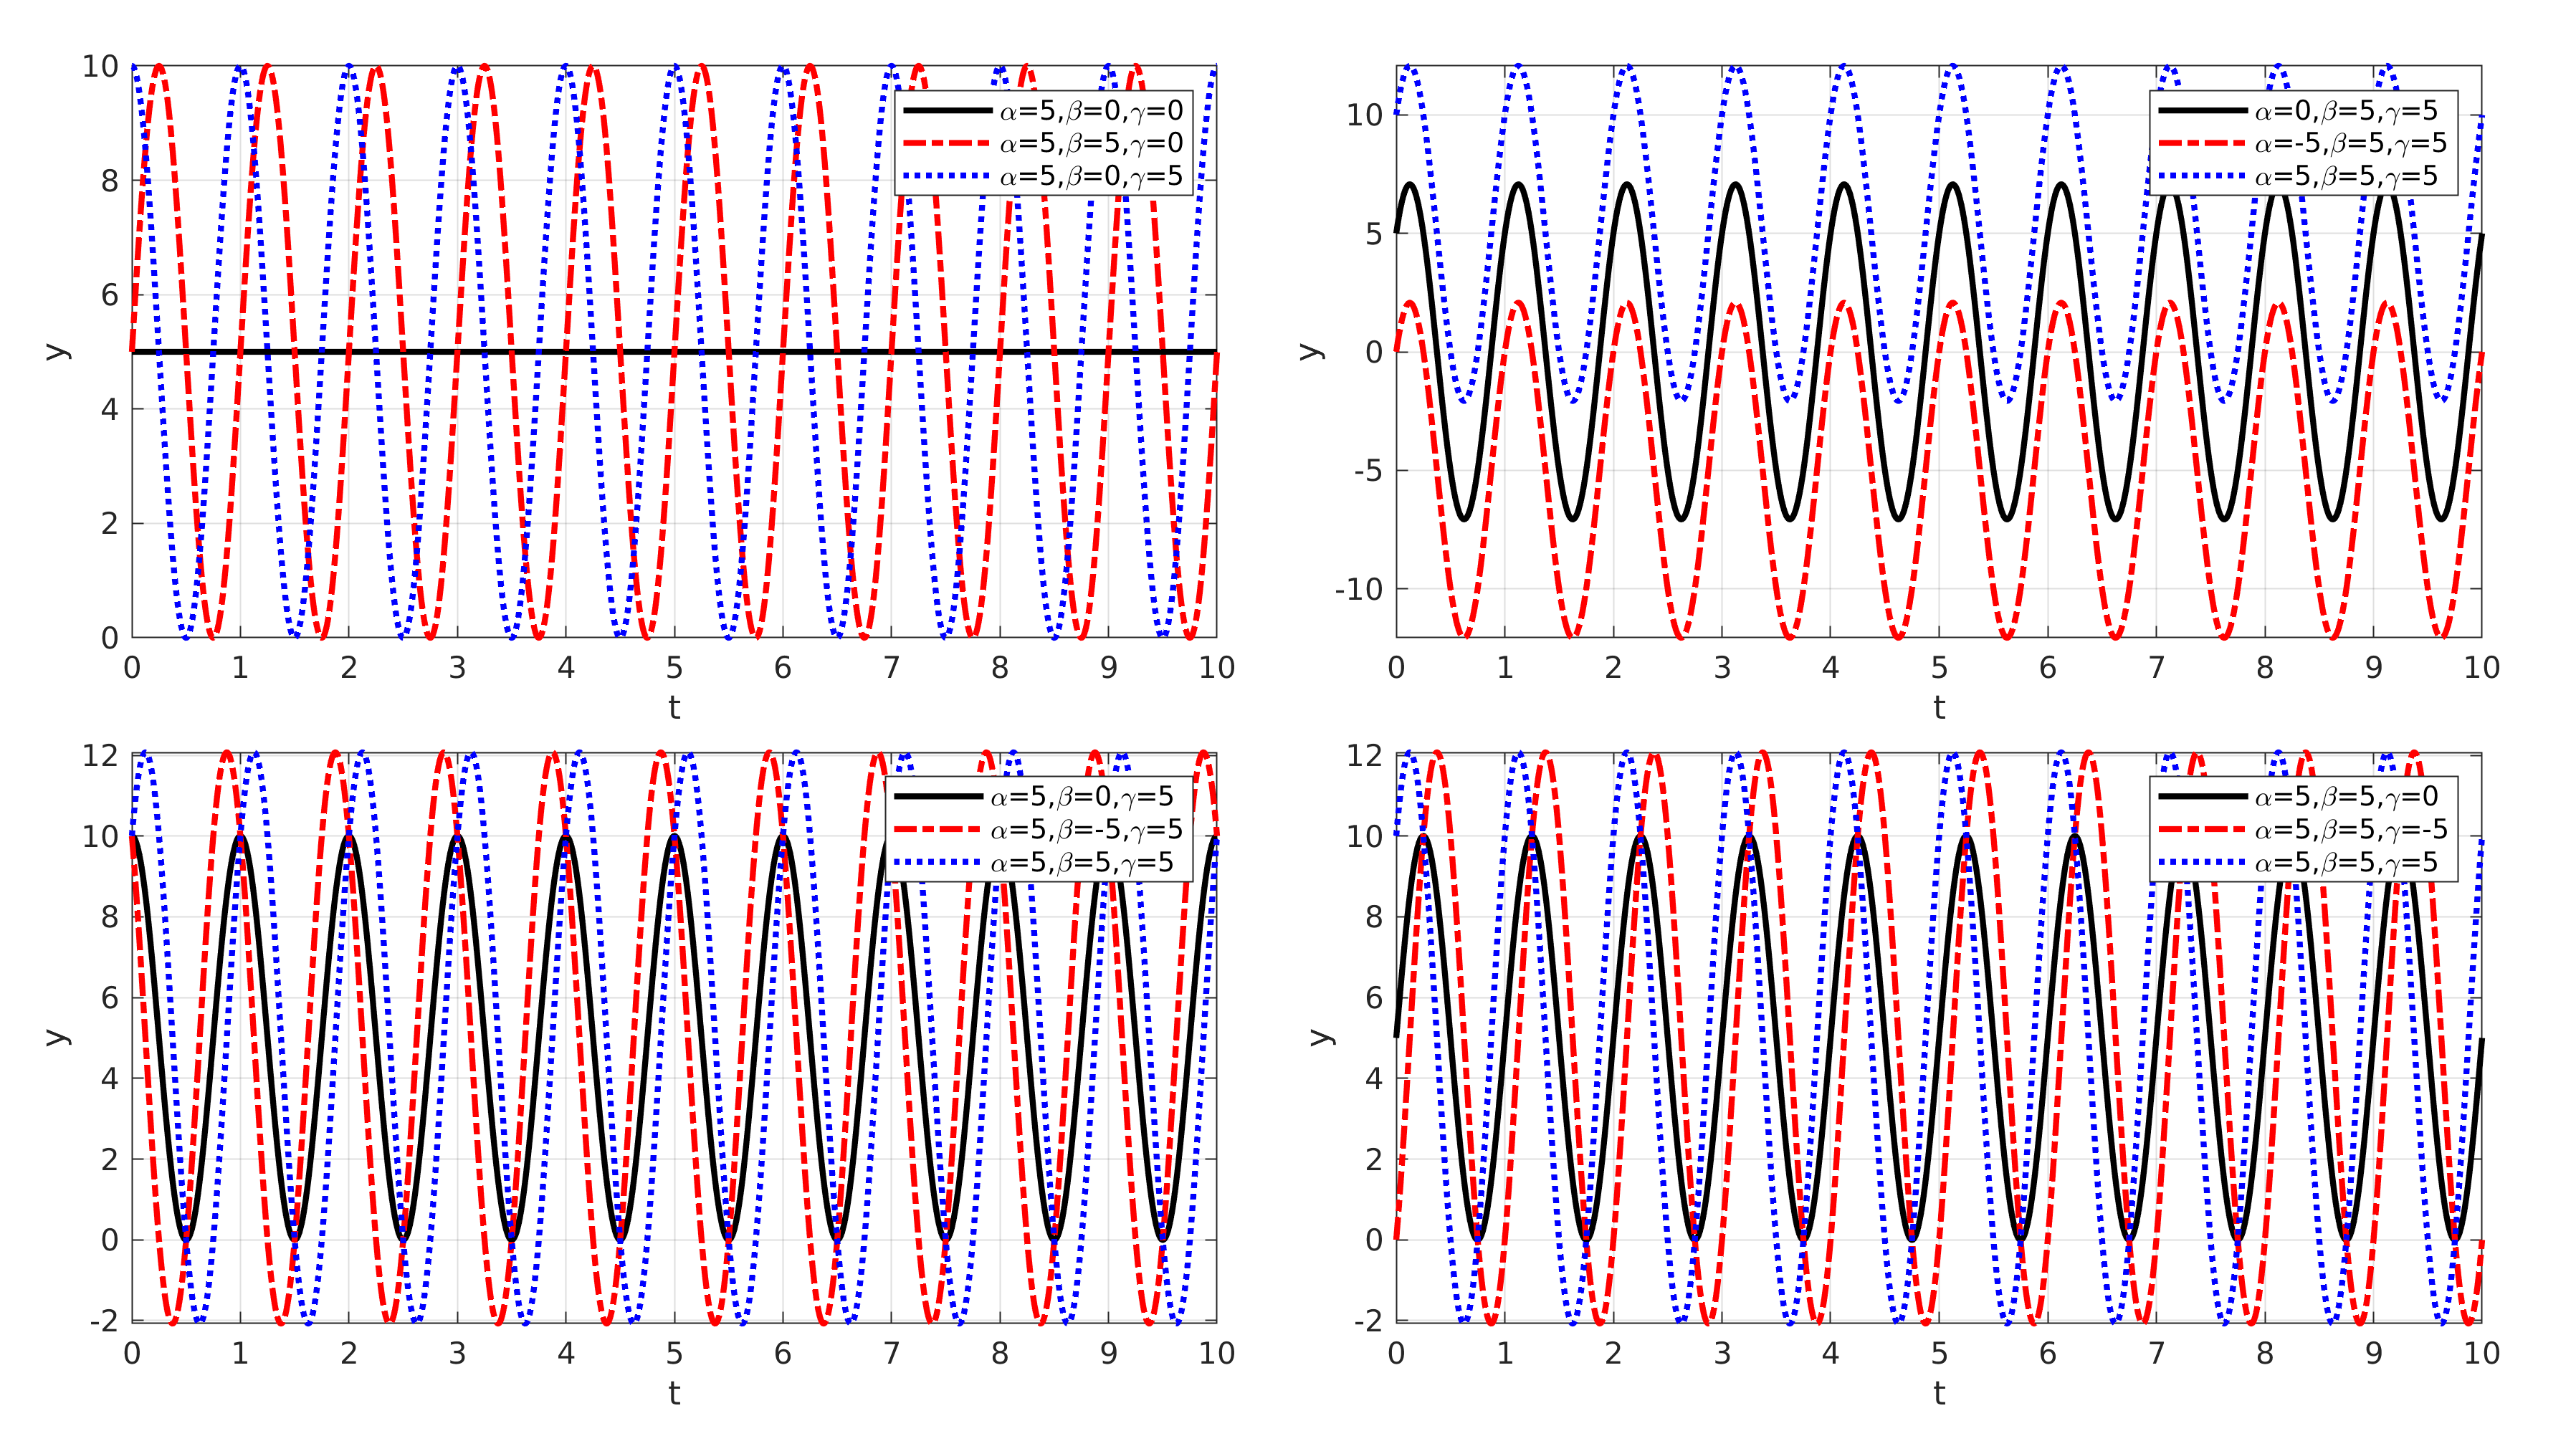
\includegraphics[width=15cm]{contents/sm_experiment}
		\caption{Kurva persamaan siklus musiman untuk beberapa nilai $\alpha,\beta$ dan $\gamma$.}
		\label{fig:sm}
	\end{figure}
	Gambar \ref{fig:sm} menampilkan ilustrasi persamaan \ref{eq:sm_} untuk nilai $\alpha,\beta$ dan $\gamma$ yang berbeda. Nilai $\alpha$ yang berbeda mempengaruhi posisi kurva terhadap sumbu-y. Sedangkan nilai $\beta$ dan $\gamma$ yang berbeda mempengaruhi posisi kurva terhadap sumbu-x.
\end{spacing}


%=====================================================================
% BAB III
\chapter{METODOLOGI PENELITIAN}
\vspace{1.5pc}
\section[Domain Penelitian]{Domain Penelitian}
\begin{spacing}{1.5}
	Domain penelitian meliputi wilayah perairan Aceh, Selat Malaka, Bagian Laut Cina Selatan dengan koordinat $-6.22^\circ-6.8^\circ$ LU dan $89.1^\circ-106.6^\circ$ BT (lihat Gambar \ref{fig:domain}) dan Teluk Benggala dengan koordinat $5.5^\circ-24.6^\circ$ LU dan $78.2^\circ-96.7^\circ$ BT (lihat Gambar \ref{fig:domain_1}). Data batimetri untuk domain penelitian diperoleh dari SRTM15+ \href{https://topex.ucsd.edu/pub/archive/srtm15/V1/}{(https://topex.ucsd.edu/)} - kisi elevasi global yang diperbarui pada interval pengambilan sampel spasial 15 arc-second (ukuran piksel $\sim 500 \times 500$ m di ekuator) \shortcite{Tozer2019}. Penelitian ini dilakukan dengan mengkaji variabilitas lapisan vertikal berdasarkan data meteorology dan aplikasinya di beberapa domain penelitian. Pertimbangan domain ini bertujuan untuk melihat keberlakukan secara umum, terhadap teori iklim dan MLD, oleh karena itu perlu diterapkan aplikasi di beberapa tempat seperti: BoB, Perairan Aceh, Selat Malaka, dan Bagian Laut Cina Selatan.
	\begin{figure}[H]
		\centering
		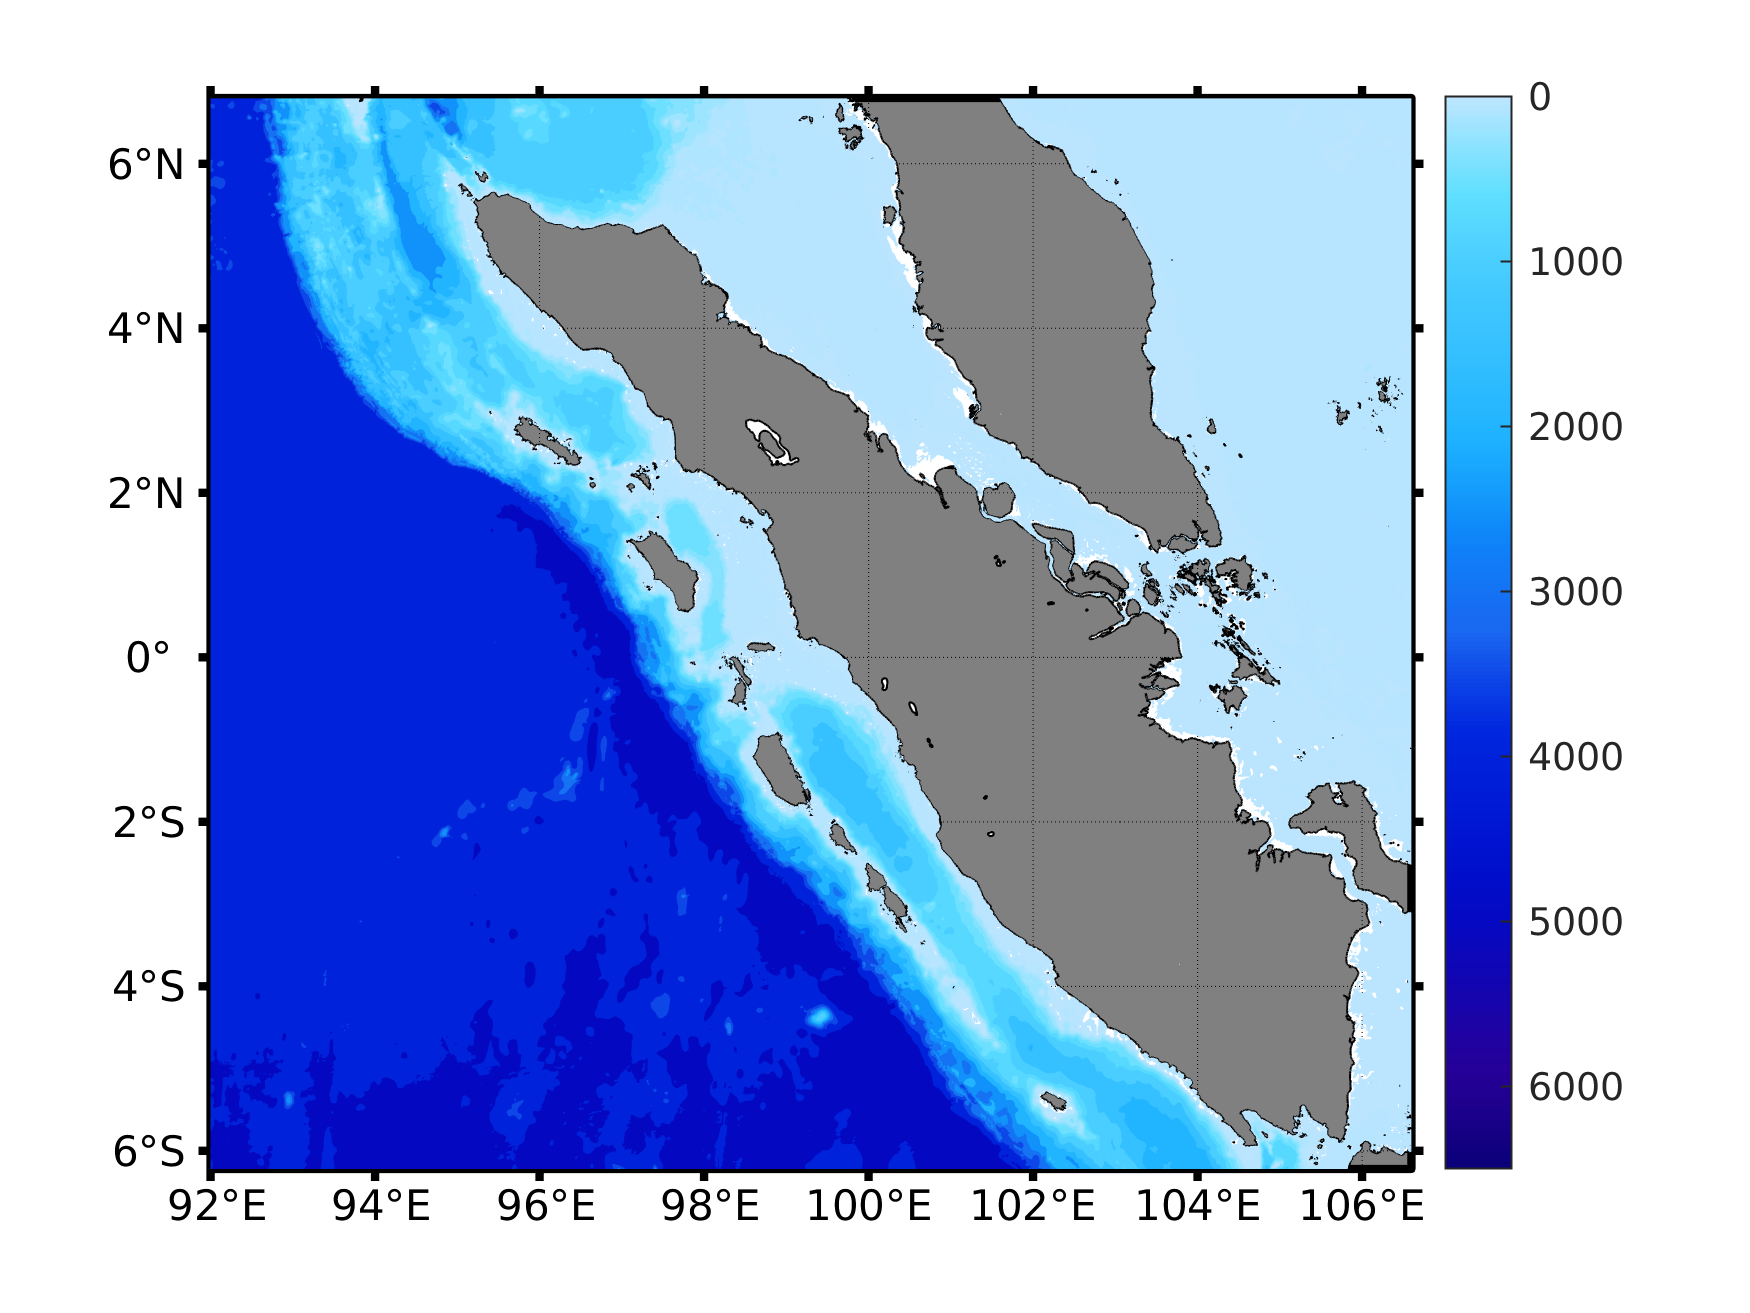
\includegraphics[width=12cm]{contents/Topo_1}
		\caption{Data batimetri domain perairan Aceh, Selat Malaka, Bagian Laut Cina Selatan, dicuplik dari SRTM15+}
		\label{fig:domain}
	\end{figure}
	\begin{figure}[H]
		\centering
		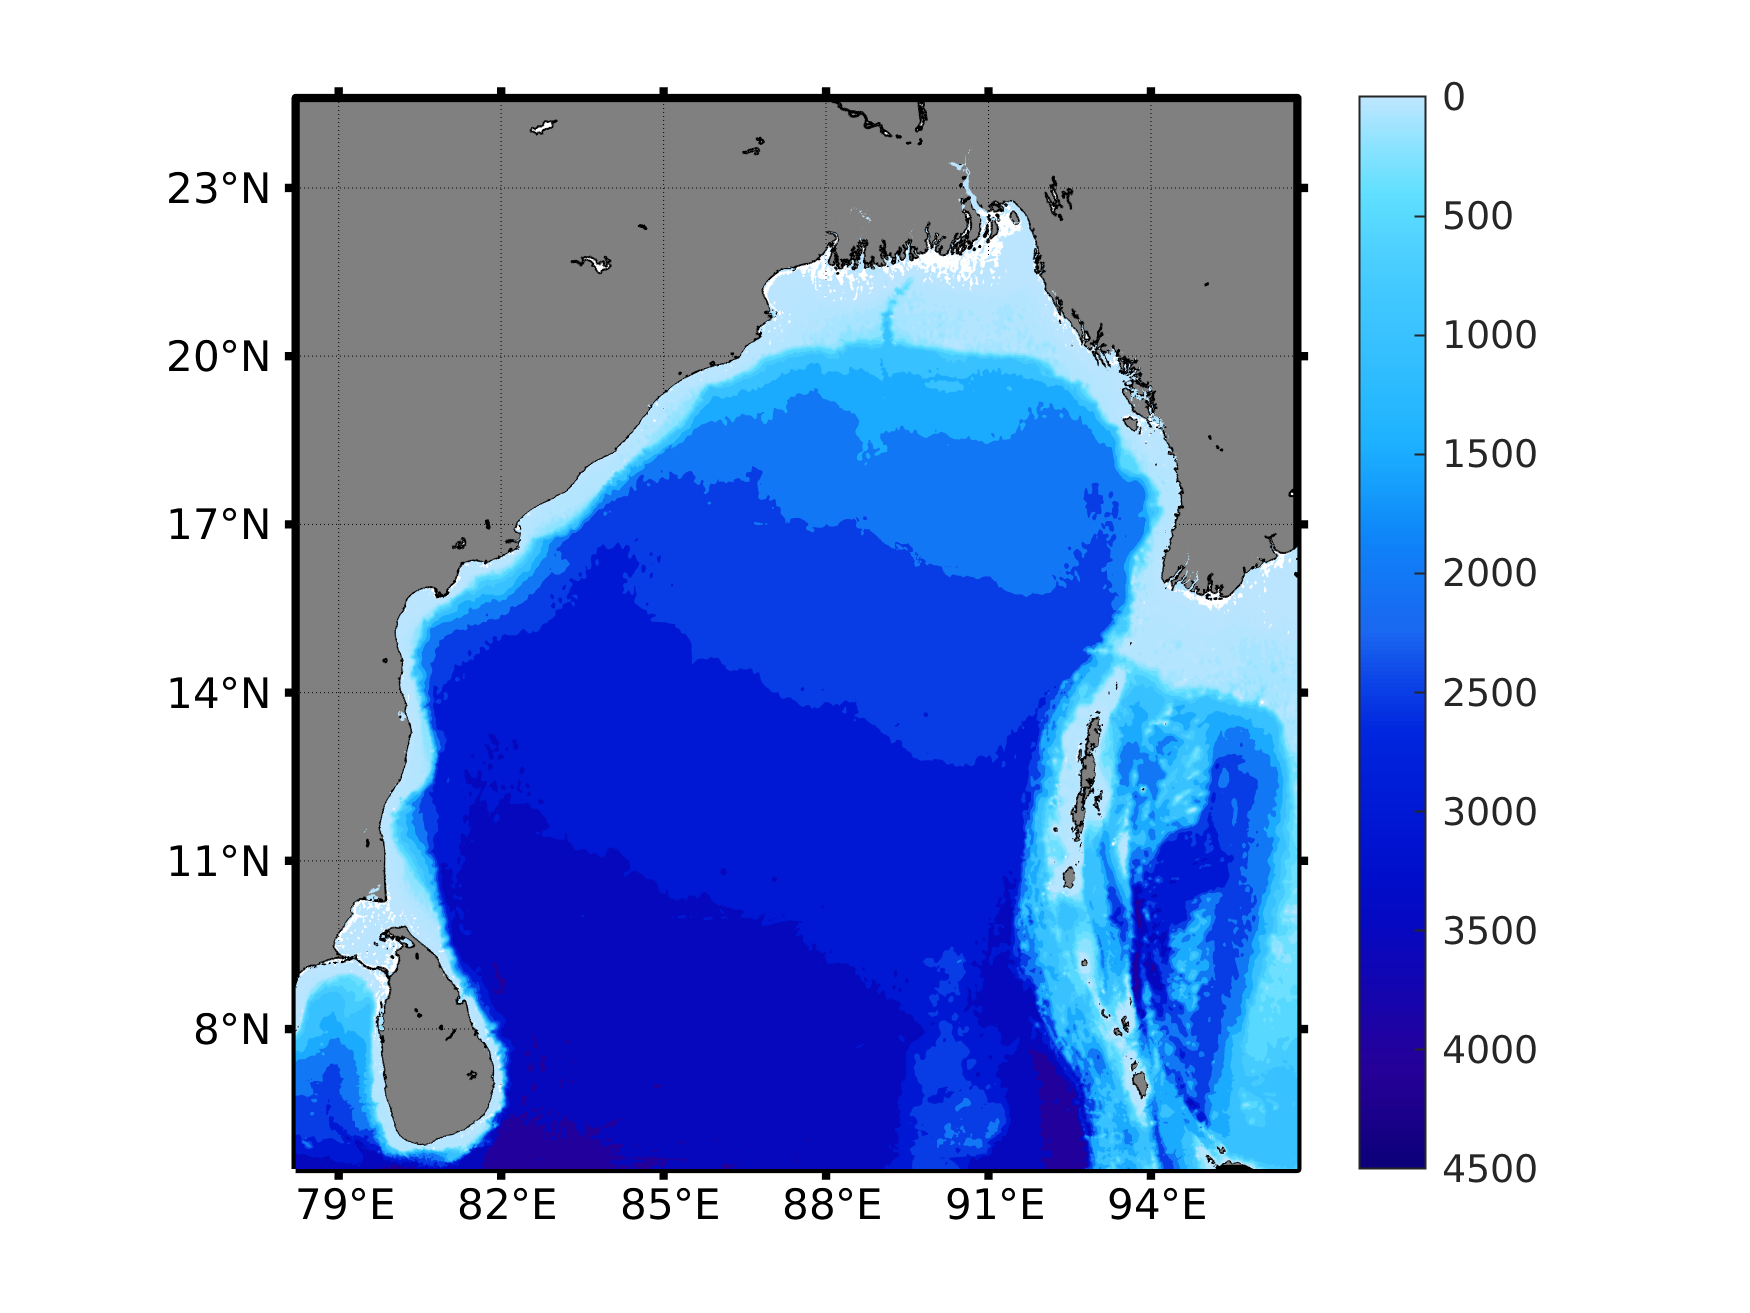
\includegraphics[width=12cm]{contents/Topo_2}
		\caption{Data batimetri domain Teluk Benggala, dicuplik dari SRTM15+}
		\label{fig:domain_1}
	\end{figure}
%	\begin{table}[htp]
%		\centering
%		\caption{Stasiun Penelitian}
%		\label{table:stasiun}
%		\begin{tabular}{ll}
%			Stasiun & Koordinat \\ \hline
%			$1$ & $3.25^\circ \text{LU}, 94^\circ \text{BT}$ \\
%			$2$ & $3.25^\circ \text{LU}, 95^\circ \text{BT}$ \\
%			$3$ & $3.25^\circ \text{LU}, 97^\circ \text{BT}$ \\
%			$4$ & $4.5^\circ \text{LU}, 94^\circ \text{BT}$ \\
%			$5$ & $4.5^\circ \text{LU}, 95^\circ \text{BT}$ \\
%			$6$ & $6^\circ \text{LU}, 94^\circ \text{BT}$ \\
%			$7$ & $6^\circ \text{LU}, 95^\circ \text{BT}$ \\
%			$8$ & $6^\circ \text{LU}, 97^\circ \text{BT}$ 
%		\end{tabular}
%	\end{table}
\end{spacing}
\vspace{-1pc}
\section[Data Penelitian]{Data Penelitian}
\begin{spacing}{1.5}
\vspace{-1pc}
\subsection[Data Oseanografi]{Data Oseanografi}
	Data oseanografi yang digunakan adalah data arus permukaan, serta data temperatur dari NEMO (\textit{Nucleus for European Modeling of the Ocean}) yang merupakan salah satu model sirkulasi laut (OGCM) yang menggunakan model numerik tiga dimensi Navier-Stokes. Model NEMO adalah model komputasi resolusi tinggi yang digunakan untuk kegiatan penelitian dan layanan peramalan dalam oseanografi dan klimatologi, yang dikembangkan secara berkelanjutan sejak 2008 oleh konsorsium Eropa yang terdiri dari 5 institusi (CMCC | CNRS | Mercator Ocean | Met Office | NERC). Hal ini dimaksudkan untuk menjadi alat yang fleksibel untuk mempelajari fenomena fisik dan biogeokimia dalam sirkulasi laut, serta interaksinya dengan komponen sistem iklim Bumi, pada berbagai skala ruang dan waktu \shortcite{madec_gurvan_2022_6334656}. 
	
	Penelitian ini menggunakan data output model NEMO (\href{https://www.nemo-ocean.eu/}{https://www.nemo-ocean.eu/}) untuk data analisis global temperatur tiga dimensi yang didownload dari website \href{https://resources.marine.copernicus.eu/products}{CMEMS} selama 12 bulan (Januari - Desember) tahun 2021.  Dalam analisis kami, resolusi data output yang digunakan adalah dx = dy = 5 menit pada bidang horizontal dan 50-lapisan $(k \in [1,50])$ dengan ketebalan berbeda pada bidang vertikal:
	\begin{equation*}
		\begin{aligned}
			z_k = \{0.49, 1.54, 2.65, 3.82, 5.08, 6.44, 7.93, 9.57, 11.40, 13.47, 15.82, 18.50, \\
			21.60, 25.21, 29.44, 34.43, 40.34, 47.37, 55.76, 65.81, 77.85, 92.33, 109.73, 130.67, \\
			155.85, 186.12, 222.47, 266.04, 318.13, 380.21, 453.94, 541.089, 643.57, 763.33, \\
			902.34, 1062.44, 1245.29, 1452.25, 1684.28, 1941.89, 2225.08, 2533.33, 2865.70,  \\
			3220.82, 3597.03, 3992.48, 4405.22, 4833.29, 5274.78, 5727.92 \} (m). \\
		\end{aligned}
	\end{equation*}
\subsection[Data Meteorologi]{Data Meteorologi}
	Data meteorologi yang digunakan adalah data reanalysis NCEP/NCAR per 6 jam \href{https://psl.noaa.gov/data/gridded/data.ncep.reanalysis.html}{(https://psl.noaa.gov/data/gridded/data.ncep.reanalysis.html)} selama 22 tahun dari tahun 2000 sampai 2021 untuk 6 parameter yaitu: \textit{2m air temperature, 2m specific humidity, convective precipitation rate, sea level pressure, wind stress U}, dan \textit{wind stress V}.
\end{spacing}
\vspace{-0.5pc}
\section[Prosedur Penelitian]{Prosedur Penelitian}
\begin{spacing}{1.5}
	\begin{figure}[H]
		\centering
		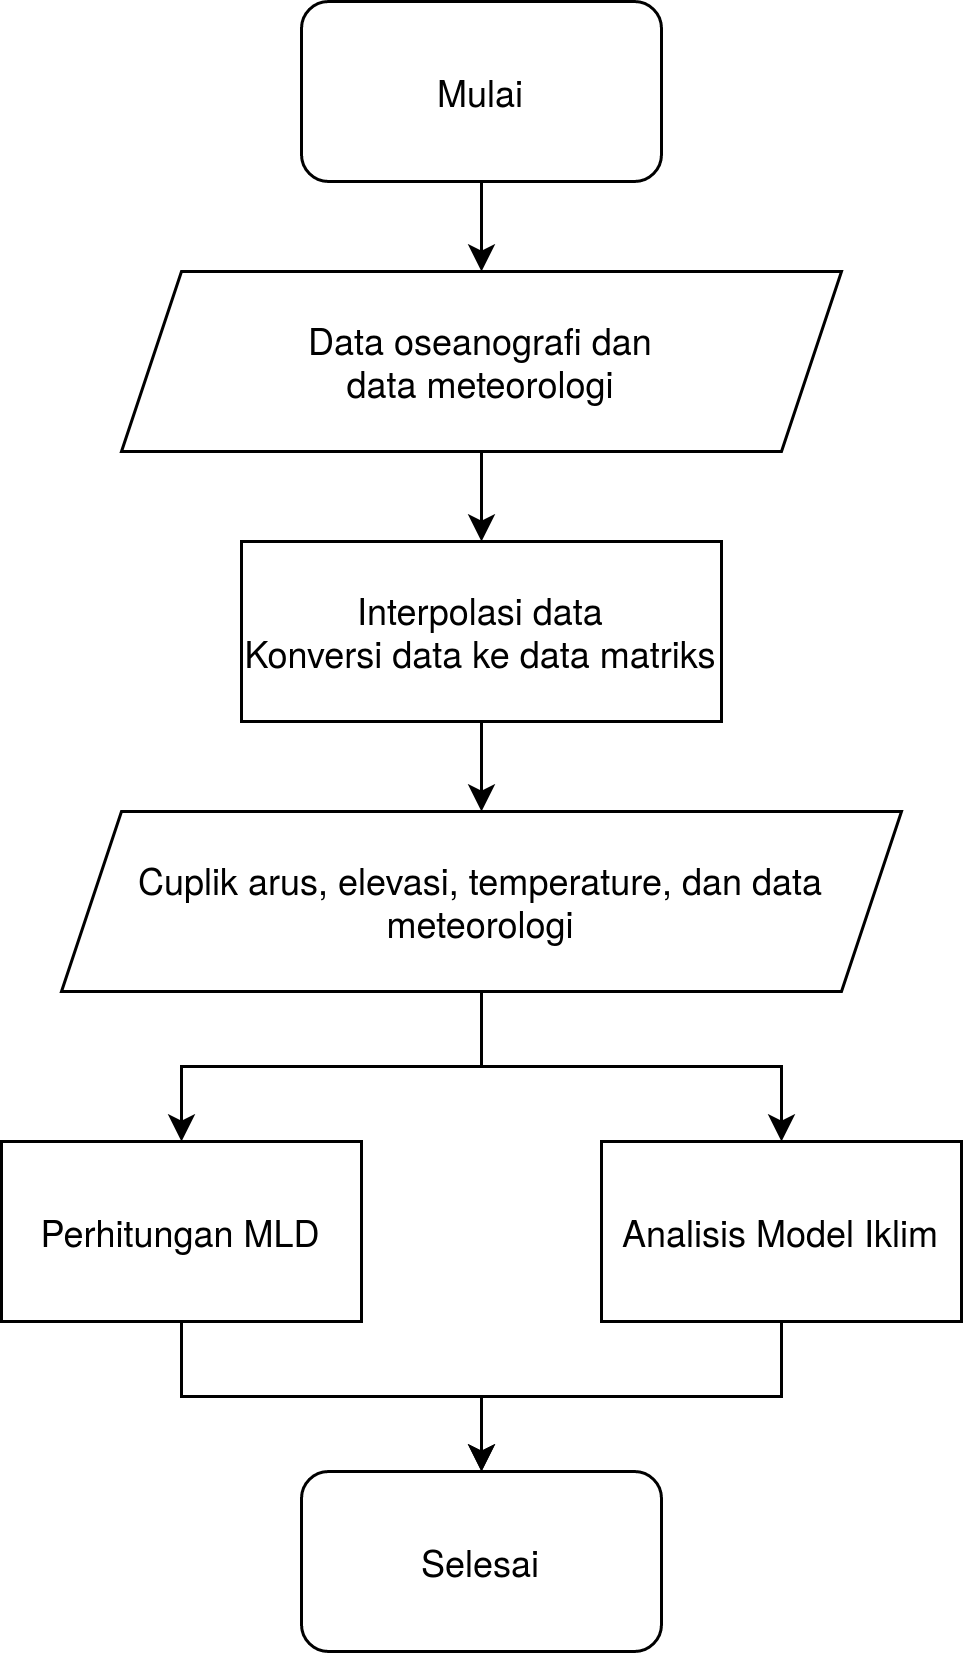
\includegraphics[width=7cm]{contents/flowchart.png}
		\caption{Diagram alir penelitian}
		\label{fig:flowchart}
	\end{figure}
	Prosedur penelitian mengikuti diagram alir pada Gambar \ref{fig:flowchart}. Data-data terkait penelitian didownload terlebih dahulu kemudian diinterpolasi untuk memenuhi data yang kosong serta untuk memperoleh resolusi spasial yang lebih detail. Selanjutnya data hasil interpolasi kemudian dibaca dan di konversi ke dalam data matriks pada MATLAB. Hasilnya adalah peta arus, elevasi, temperature, dan data meteorologi. Peta temperature kemudian diobservasi untuk menentukan kedalaman lapisan campuran selama 12 bulan. Sebagai verifikasi atas observasi kedalaman lapisan campuran, akan dilakukan analisis model iklim terhadap data meteorologi (\textit{2m air temperature, 2m specific humidity, convective precipitation rate, sea level pressure, wind stress U}, dan \textit{wind stress V}) selama 22 tahun dari tahun 2000 sampai 2021.
\end{spacing}
%=====================================================================
% Halaman Output
\pagebreak
\chapter{BIAYA DAN JADWAL PENELITIAN}
\vspace{1.5pc}
\section[Biaya Penelitian]{Biaya Penelitian}
\begin{spacing}{1.5}
	Anggaran biaya penelitian dapat dilihat pada tabel berikut:
	% Please add the following required packages to your document preamble:
	% \usepackage[normalem]{ulem}
	% \useunder{\uline}{\ul}{}
	\begin{table}[htp]
		\caption{Ringkasan anggaran biaya penelitian}
		\label{tab:ang-pen}
		\begin{tabular}{|ll|l|}
			\hline
			\multicolumn{1}{|l|}{No} & Jenis Pengeluaran                                                                                                                                                                                        & \begin{tabular}[c]{@{}l@{}}Biaya yang \\ diusulkan (Rp)\end{tabular} \\ \hline
			\multicolumn{1}{|l|}{1}  & \begin{tabular}[c]{@{}l@{}}Honorarium untuk pelaksana, petugas laboratorium, \\ pengumpul data, pengolah data, dan penganalisis data.\end{tabular}                                                       & 10.000.000                                                           \\ \hline
			\multicolumn{1}{|l|}{2}  & \begin{tabular}[c]{@{}l@{}}Pembelian bahan habis pakai untuk ATK, fotocopy, \\ surat menyurat, penyusunan laporan, cetak, penjilidan,\\ publikasi, pulsa, internet, dan bahan laboratorium.\end{tabular} & 40.000.000                                                           \\ \hline
			\multicolumn{1}{|l|}{3}  & \begin{tabular}[c]{@{}l@{}}Perjalanan untuk biaya survei/sampling data, seminar/\\ workshop DN-LN, biaya akomodasi, konsumsi, \\ perdiem/lumpsum, transport.\end{tabular}                                & 10.000.000                                                           \\ \hline
			\multicolumn{1}{|l|}{4}  & \begin{tabular}[c]{@{}l@{}}Sewa untuk peralatan/mesin/ruang laboratorium, \\ kendaraan, dan peralatan penunjang penelitian lainnya.\end{tabular}                                                         & 0                                                                    \\ \hline
			\multicolumn{2}{|c|}{Total}                                                                                                                                                                                                         & 60.000.000                                                           \\ \hline
		\end{tabular}
	\end{table}
\end{spacing}
%\vspace{-0.5pc}
\pagebreak 
\section[Jadwal Penelitian]{Jadwal Penelitian}
\begin{spacing}{1.5}
	Jadwal penelitian disusun berdasarkan lama studi yang telah ditempuh dan akan ditempuh. Penelitian diusulkan dalam tiga tahun, dengan rincian kegiatan sebagai berikut:
	% Please add the following required packages to your document preamble:
	% \usepackage{multirow}
	% \usepackage[table,xcdraw]{xcolor}
	% If you use beamer only pass "xcolor=table" option, i.e. \documentclass[xcolor=table]{beamer}
	\begin{table}[htp]
		\caption{Ringkasan jadwal pelaksanaan penelitian}
		\label{tab:jad-pen}
		\begin{tabular}{|l|l|llllllllllll|}
			\hline
			\multicolumn{1}{|c|}{}                     &                                                                                      & \multicolumn{12}{c|}{Tahun I}                                                                                                                                                                                                                                                                                                                                                                                                                                                                                                                                            \\ \cline{3-14} 
			\multicolumn{1}{|c|}{\multirow{-2}{*}{No}} & \multirow{-2}{*}{Kegiatan}                                                           & \multicolumn{1}{c|}{1}                        & \multicolumn{1}{c|}{2}                        & \multicolumn{1}{c|}{3}                        & \multicolumn{1}{c|}{4}                        & \multicolumn{1}{c|}{5}                        & \multicolumn{1}{c|}{6}                        & \multicolumn{1}{c|}{7}                        & \multicolumn{1}{c|}{8}                        & \multicolumn{1}{c|}{9}                        & \multicolumn{1}{c|}{10}                       & \multicolumn{1}{c|}{11}                       & \multicolumn{1}{c|}{12}  \\ \hline
			1                                          & Studi literatur                                                                      & \multicolumn{1}{l|}{\cellcolor[HTML]{343434}} & \multicolumn{1}{l|}{\cellcolor[HTML]{343434}} & \multicolumn{1}{l|}{\cellcolor[HTML]{343434}} & \multicolumn{1}{l|}{\cellcolor[HTML]{343434}} & \multicolumn{1}{l|}{}                         & \multicolumn{1}{l|}{}                         & \multicolumn{1}{l|}{}                         & \multicolumn{1}{l|}{}                         & \multicolumn{1}{l|}{}                         & \multicolumn{1}{l|}{}                         & \multicolumn{1}{l|}{}                         &                          \\ \hline
			2                                          & Penyusunan proposal                                                                  & \multicolumn{1}{l|}{}                         & \multicolumn{1}{l|}{}                         & \multicolumn{1}{l|}{}                         & \multicolumn{1}{l|}{}                         & \multicolumn{1}{l|}{\cellcolor[HTML]{343434}} & \multicolumn{1}{l|}{\cellcolor[HTML]{343434}} & \multicolumn{1}{l|}{\cellcolor[HTML]{343434}} & \multicolumn{1}{l|}{\cellcolor[HTML]{343434}} & \multicolumn{1}{l|}{}                         & \multicolumn{1}{l|}{}                         & \multicolumn{1}{l|}{}                         &                          \\ \hline
			3                                          & \begin{tabular}[c]{@{}l@{}}Persiapan data model \\ dan data observasi\end{tabular}   & \multicolumn{1}{l|}{}                         & \multicolumn{1}{l|}{}                         & \multicolumn{1}{l|}{}                         & \multicolumn{1}{l|}{}                         & \multicolumn{1}{l|}{}                         & \multicolumn{1}{l|}{}                         & \multicolumn{1}{l|}{}                         & \multicolumn{1}{l|}{}                         & \multicolumn{1}{l|}{\cellcolor[HTML]{343434}} & \multicolumn{1}{l|}{\cellcolor[HTML]{343434}} & \multicolumn{1}{l|}{\cellcolor[HTML]{343434}} &                          \\ \hline
			4                                          & Pemrosesan data                                                                      & \multicolumn{1}{l|}{}                         & \multicolumn{1}{l|}{}                         & \multicolumn{1}{l|}{}                         & \multicolumn{1}{l|}{}                         & \multicolumn{1}{l|}{}                         & \multicolumn{1}{l|}{}                         & \multicolumn{1}{l|}{}                         & \multicolumn{1}{l|}{}                         & \multicolumn{1}{l|}{}                         & \multicolumn{1}{l|}{}                         & \multicolumn{1}{l|}{}                         & \cellcolor[HTML]{343434} \\ \hline
			\multicolumn{1}{|c|}{}                     &                                                                                      & \multicolumn{12}{c|}{Tahun II}                                                                                                                                                                                                                                                                                                                                                                                                                                                                                                                                           \\ \cline{3-14} 
			\multicolumn{1}{|c|}{\multirow{-2}{*}{No}} & \multirow{-2}{*}{Kegiatan}                                                           & \multicolumn{1}{c|}{1}                        & \multicolumn{1}{c|}{`2}                       & \multicolumn{1}{c|}{3}                        & \multicolumn{1}{c|}{4}                        & \multicolumn{1}{c|}{5}                        & \multicolumn{1}{c|}{6}                        & \multicolumn{1}{c|}{7}                        & \multicolumn{1}{c|}{8}                        & \multicolumn{1}{c|}{9}                        & \multicolumn{1}{c|}{10}                       & \multicolumn{1}{c|}{11}                       & \multicolumn{1}{c|}{12}  \\ \hline
			5                                          & Pemrosesan data lanjutan                                                             & \multicolumn{1}{l|}{\cellcolor[HTML]{343434}} & \multicolumn{1}{l|}{\cellcolor[HTML]{343434}} & \multicolumn{1}{l|}{}                         & \multicolumn{1}{l|}{}                         & \multicolumn{1}{l|}{}                         & \multicolumn{1}{l|}{}                         & \multicolumn{1}{l|}{}                         & \multicolumn{1}{l|}{}                         & \multicolumn{1}{l|}{}                         & \multicolumn{1}{l|}{}                         & \multicolumn{1}{l|}{}                         &                          \\ \hline
			6                                          & Hasil dan analisis                                                                   & \multicolumn{1}{l|}{}                         & \multicolumn{1}{l|}{}                         & \multicolumn{1}{l|}{\cellcolor[HTML]{343434}} & \multicolumn{1}{l|}{\cellcolor[HTML]{343434}} & \multicolumn{1}{l|}{}                         & \multicolumn{1}{l|}{}                         & \multicolumn{1}{l|}{}                         & \multicolumn{1}{l|}{}                         & \multicolumn{1}{l|}{}                         & \multicolumn{1}{l|}{}                         & \multicolumn{1}{l|}{}                         &                          \\ \hline
			7                                          & Publikasi 1                                                                          & \multicolumn{1}{l|}{}                         & \multicolumn{1}{l|}{}                         & \multicolumn{1}{l|}{}                         & \multicolumn{1}{l|}{}                         & \multicolumn{1}{l|}{\cellcolor[HTML]{343434}} & \multicolumn{1}{l|}{\cellcolor[HTML]{343434}} & \multicolumn{1}{l|}{\cellcolor[HTML]{343434}} & \multicolumn{1}{l|}{}                         & \multicolumn{1}{l|}{}                         & \multicolumn{1}{l|}{}                         & \multicolumn{1}{l|}{}                         &                          \\ \hline
			8                                          & Studi literatur lanjutan                                                             & \multicolumn{1}{l|}{}                         & \multicolumn{1}{l|}{}                         & \multicolumn{1}{l|}{}                         & \multicolumn{1}{l|}{}                         & \multicolumn{1}{l|}{}                         & \multicolumn{1}{l|}{}                         & \multicolumn{1}{l|}{}                         & \multicolumn{1}{l|}{\cellcolor[HTML]{343434}} & \multicolumn{1}{l|}{\cellcolor[HTML]{343434}} & \multicolumn{1}{l|}{\cellcolor[HTML]{343434}} & \multicolumn{1}{l|}{}                         &                          \\ \hline
			9                                          & Hasil dan analisis                                                                   & \multicolumn{1}{l|}{}                         & \multicolumn{1}{l|}{}                         & \multicolumn{1}{l|}{}                         & \multicolumn{1}{l|}{}                         & \multicolumn{1}{l|}{}                         & \multicolumn{1}{l|}{}                         & \multicolumn{1}{l|}{}                         & \multicolumn{1}{l|}{}                         & \multicolumn{1}{l|}{}                         & \multicolumn{1}{l|}{\cellcolor[HTML]{343434}} & \multicolumn{1}{l|}{\cellcolor[HTML]{343434}} & \cellcolor[HTML]{343434} \\ \hline
			\multicolumn{1}{|c|}{}                     &                                                                                      & \multicolumn{12}{c|}{Tahun III}                                                                                                                                                                                                                                                                                                                                                                                                                                                                                                                                          \\ \cline{3-14} 
			\multicolumn{1}{|c|}{\multirow{-2}{*}{No}} & \multirow{-2}{*}{Kegiatan}                                                           & \multicolumn{1}{c|}{1}                        & \multicolumn{1}{c|}{2}                        & \multicolumn{1}{c|}{3}                        & \multicolumn{1}{c|}{4}                        & \multicolumn{1}{c|}{5}                        & \multicolumn{1}{c|}{6}                        & \multicolumn{1}{c|}{7}                        & \multicolumn{1}{c|}{8}                        & \multicolumn{1}{c|}{9}                        & \multicolumn{1}{c|}{10}                       & \multicolumn{1}{c|}{11}                       & \multicolumn{1}{c|}{12}  \\ \hline
			10                                         & Publikasi 2                                                                          & \multicolumn{1}{l|}{\cellcolor[HTML]{343434}} & \multicolumn{1}{l|}{\cellcolor[HTML]{343434}} & \multicolumn{1}{l|}{\cellcolor[HTML]{343434}} & \multicolumn{1}{l|}{\cellcolor[HTML]{343434}} & \multicolumn{1}{l|}{}                         & \multicolumn{1}{l|}{}                         & \multicolumn{1}{l|}{}                         & \multicolumn{1}{l|}{}                         & \multicolumn{1}{l|}{}                         & \multicolumn{1}{l|}{}                         & \multicolumn{1}{l|}{}                         &                          \\ \hline
			11                                         & \begin{tabular}[c]{@{}l@{}}Studi literatur untuk \\ penulisan disertasi\end{tabular} & \multicolumn{1}{l|}{}                         & \multicolumn{1}{l|}{}                         & \multicolumn{1}{l|}{}                         & \multicolumn{1}{l|}{}                         & \multicolumn{1}{l|}{\cellcolor[HTML]{343434}} & \multicolumn{1}{l|}{\cellcolor[HTML]{343434}} & \multicolumn{1}{l|}{\cellcolor[HTML]{343434}} & \multicolumn{1}{l|}{}                         & \multicolumn{1}{l|}{}                         & \multicolumn{1}{l|}{}                         & \multicolumn{1}{l|}{}                         &                          \\ \hline
			12                                         & Penyusunan disertasi                                                                 & \multicolumn{1}{l|}{}                         & \multicolumn{1}{l|}{}                         & \multicolumn{1}{l|}{}                         & \multicolumn{1}{l|}{}                         & \multicolumn{1}{l|}{}                         & \multicolumn{1}{l|}{}                         & \multicolumn{1}{l|}{}                         & \multicolumn{1}{l|}{\cellcolor[HTML]{343434}} & \multicolumn{1}{l|}{\cellcolor[HTML]{343434}} & \multicolumn{1}{l|}{}                         & \multicolumn{1}{l|}{}                         &                          \\ \hline
		\end{tabular}
	\end{table}
\end{spacing}
%=====================================================================
% BAB IV
%\chapter{HASIL DAN PEMBAHASAN}
%\vspace{1.5pc}
\vspace{1.5pc}
\section[Hasil 1]{HASIL 1}
\begin{spacing}{1.5}
	
	\lipsum[1-4]
	
\end{spacing}
%=====================================================================
% BAB V
%\chapter{PENUTUP}
%\vspace{1.5pc}
\vspace{1.5pc}
\begin{spacing}{1.5}
\section[Kesimpulan]{KESIMPULAN}

\lipsum[2-4]

\section[Saran]{SARAN}

\lipsum[2-4]\cite{Adams2011}

\end{spacing}
%=====================================================================
% Halaman Daftar Pustaka
\pagebreak
%\addcontentsline{toc}{chapter}{\textbf{DAFTAR PUSTAKA}}
\renewcommand\bibname{DAFTAR PUSTAKA}	
\bibliographystyle{packages/apacite}
\bibliography{contents/ReferenceMendeley.bib}
%\{DAFTAR}
%=====================================================================
% Halaman Lampiran
%\newpage
%\newappendix{Lampiran 1. Listing Program}
%\addcontentsline{toc}{chapter}{LAMPIRAN}
%% Please add the following required packages to your document preamble:
% \usepackage{graphicx}
\begin{table}[H]
%	\caption{}
	\label{tab:just-anggaran}
	\resizebox{\textwidth}{!}{%
		\begin{tabular}{|lllll|}
			\hline
			\multicolumn{5}{|l|}{\textbf{1. Honorarium}}                                                                                                                                                                                                                                                                                                                                                                                                                                                                                                           \\ \hline
			\multicolumn{1}{|c|}{Honor}                                                                                  & \multicolumn{1}{c|}{\begin{tabular}[c]{@{}c@{}}Honor/Jam \\ (Rp)\end{tabular}}                                                                          & \multicolumn{1}{c|}{\begin{tabular}[c]{@{}c@{}}Waktu \\ (Jam/Minggu)\end{tabular}} & \multicolumn{1}{c|}{Minggu}                                                          & \multicolumn{1}{c|}{\begin{tabular}[c]{@{}c@{}}Honor per Tahun\\ (Rp)\end{tabular}}               \\ \hline
			\multicolumn{1}{|l|}{Teknisi 1}                                                                              & \multicolumn{1}{l|}{25.000}                                                                                                                             & \multicolumn{1}{l|}{5}                                                             & \multicolumn{1}{l|}{20}                                                              & 2.500.000                                                                                         \\ \hline
			\multicolumn{1}{|l|}{Teknisi 2}                                                                              & \multicolumn{1}{l|}{25.000}                                                                                                                             & \multicolumn{1}{l|}{5}                                                             & \multicolumn{1}{l|}{20}                                                              & 2.500.000                                                                                         \\ \hline
			\multicolumn{1}{|l|}{Pengolah data}                                                                          & \multicolumn{1}{l|}{50.000}                                                                                                                             & \multicolumn{1}{l|}{6}                                                             & \multicolumn{1}{l|}{5}                                                               & 1.500.000                                                                                         \\ \hline
			\multicolumn{1}{|l|}{Sekretariat}                                                                            & \multicolumn{1}{l|}{25.000}                                                                                                                             & \multicolumn{1}{l|}{5}                                                             & \multicolumn{1}{l|}{24}                                                              & 3.000.000                                                                                         \\ \hline
			\multicolumn{4}{|l|}{SUB TOTAL (Rp)}                                                                                                                                                                                                                                                                                                                                                                                                               & 9.500.000                                                                                         \\ \hline
			\multicolumn{5}{|l|}{\textbf{2. Pembelian Bahan Habis Pakai}}                                                                                                                                                                                                                                                                                                                                                                                                                                                                                          \\ \hline
			\multicolumn{1}{|c|}{Material}                                                                               & \multicolumn{1}{c|}{\begin{tabular}[c]{@{}c@{}}Justifikasi \\ Pemakaian\end{tabular}}                                                                   & \multicolumn{1}{c|}{Kuantitas}                                                     & \multicolumn{1}{c|}{\begin{tabular}[c]{@{}c@{}}Harga \\ Satuan \\ (Rp)\end{tabular}} & \multicolumn{1}{c|}{\begin{tabular}[c]{@{}c@{}}Harga Peralatan \\ Penunjang \\ (Rp)\end{tabular}} \\ \hline
			\multicolumn{1}{|l|}{ATK}                                                                                    & \multicolumn{1}{l|}{Bahan pendukung}                                                                                                                    & \multicolumn{1}{l|}{1 paket}                                                       & \multicolumn{1}{l|}{10.000.000}                                                      & 10.000.000                                                                                        \\ \hline
			\multicolumn{1}{|l|}{Eksternal hardisk}                                                                      & \multicolumn{1}{l|}{\begin{tabular}[c]{@{}l@{}}Penyimpanan data mentah \\ dan hasil olah data\end{tabular}}                                             & \multicolumn{1}{l|}{4 paket}                                                       & \multicolumn{1}{l|}{1.300.000}                                                       & 5.200.000                                                                                         \\ \hline
			\multicolumn{1}{|l|}{Print laporan}                                                                          & \multicolumn{1}{l|}{\begin{tabular}[c]{@{}l@{}}Pelaporan hasil dan \\ kegiatan penelitian\end{tabular}}                                                 & \multicolumn{1}{l|}{500 lembar}                                                    & \multicolumn{1}{l|}{2.000}                                                           & 1.000.000                                                                                         \\ \hline
			\multicolumn{1}{|l|}{\begin{tabular}[c]{@{}l@{}}Publikasi\\ prosiding\\ konferensi\end{tabular}}             & \multicolumn{1}{l|}{\begin{tabular}[c]{@{}l@{}}Biaya 1 paket seminar dan \\ publikasi pada prosiding\end{tabular}}                                      & \multicolumn{1}{l|}{1 kali}                                                        & \multicolumn{1}{l|}{3.000.000}                                                       & 3.000.000                                                                                         \\ \hline
			\multicolumn{1}{|l|}{Fotokopi}                                                                               & \multicolumn{1}{l|}{\begin{tabular}[c]{@{}l@{}}Penggandaan data mentah, \\ hasil analisis, dan draft\\ laporan\end{tabular}}                            & \multicolumn{1}{l|}{5000 lembar}                                                   & \multicolumn{1}{l|}{250}                                                             & 1.250.000                                                                                         \\ \hline
			\multicolumn{4}{|l|}{SUB TOTAL (Rp)}                                                                                                                                                                                                                                                                                                                                                                                                               & 23.800.000                                                                                        \\ \hline
			\multicolumn{5}{|l|}{\textbf{3. Perjalanan}}                                                                                                                                                                                                                                                                                                                                                                                                                                                                                                           \\ \hline
			\multicolumn{1}{|c|}{Material}                                                                               & \multicolumn{1}{c|}{Justifikasi Perjalanan}                                                                                                             & \multicolumn{1}{c|}{Kuantitas}                                                     & \multicolumn{1}{c|}{\begin{tabular}[c]{@{}c@{}}Harga \\ Satuan\\ (Rp)\end{tabular}}  & \multicolumn{1}{c|}{\begin{tabular}[c]{@{}c@{}}Biaya per Tahun\\ (Rp)\end{tabular}}               \\ \hline
			\multicolumn{1}{|l|}{\begin{tabular}[c]{@{}l@{}}Transportasi \\ seminar/workshop\\ DN/LN\end{tabular}}       & \multicolumn{1}{l|}{\begin{tabular}[c]{@{}l@{}}Transportasi udara dari \\ Banda Aceh ke kota tujuan \\ seminar DN/LN\end{tabular}}                      & \multicolumn{1}{l|}{1 kali PP}                                                     & \multicolumn{1}{l|}{14.000.000}                                                      & 14.000.000                                                                                        \\ \hline
			\multicolumn{1}{|l|}{\begin{tabular}[c]{@{}l@{}}Akomodasi \\ penginapan\end{tabular}}                        & \multicolumn{1}{l|}{\begin{tabular}[c]{@{}l@{}}Penginapan di hotel\\ bintang tiga/empat\end{tabular}}                                                   & \multicolumn{1}{l|}{3 malam}                                                       & \multicolumn{1}{l|}{1.100.000}                                                       & 3.300.000                                                                                         \\ \hline
			\multicolumn{1}{|l|}{\begin{tabular}[c]{@{}l@{}}Konsumsi/uang\\ saku seminar/\\ workshop DN/LN\end{tabular}} & \multicolumn{1}{l|}{\begin{tabular}[c]{@{}l@{}}Konsumsi yang tidak \\ ditanggung oleh hotel dan\\ penyelenggara seminar/\\ workshop DN/LN\end{tabular}} & \multicolumn{1}{l|}{3 hari}                                                        & \multicolumn{1}{l|}{800.000}                                                         & 2.400.000                                                                                         \\ \hline
			\multicolumn{4}{|l|}{SUB TOTAL (Rp)}                                                                                                                                                                                                                                                                                                                                                                                                               & 19.700.000                                                                                        \\ \hline
			\multicolumn{5}{|l|}{\textbf{4. Sewa}}                                                                                                                                                                                                                                                                                                                                                                                                                                                                                                                 \\ \hline
			\multicolumn{1}{|c|}{Material}                                                                               & \multicolumn{1}{c|}{Justifikasi Sewa}                                                                                                                   & \multicolumn{1}{c|}{Kuantitas}                                                     & \multicolumn{1}{c|}{\begin{tabular}[c]{@{}c@{}}Harga\\ Satuan\\ (Rp)\end{tabular}}   & \multicolumn{1}{c|}{\begin{tabular}[c]{@{}c@{}}Biaya per Tahun\\ (Rp)\end{tabular}}               \\ \hline
			\multicolumn{1}{|l|}{-}                                                                                      & \multicolumn{1}{l|}{-}                                                                                                                                  & \multicolumn{1}{l|}{-}                                                             & \multicolumn{1}{l|}{-}                                                               & 0                                                                                                 \\ \hline
			\multicolumn{4}{|l|}{SUB TOTAL (Rp)}                                                                                                                                                                                                                                                                                                                                                                                                               & 0                                                                                                 \\ \hline
			\multicolumn{4}{|l|}{TOTAL ANGGARAN YANG DIPERLUKAN SETIAP TAHUN (Rp)}                                                                                                                                                                                                                                                                                                                                                                             & 50.000.000                                                                                        \\ \hline
			\multicolumn{4}{|l|}{TOTAL ANGGARAN YANG DIPERLUKAN SELURUH TAHUN (Rp)}                                                                                                                                                                                                                                                                                                                                                                            & 150.000.000                                                                                       \\ \hline
		\end{tabular}%
	}
\end{table}
%\pagebreak
%\newappendix{Lampiran 2. Diskritisasi pada C-grid Arakawa}
%Dukungan yang memungkinkan terlaksananya penelitian ini adalah tersedianya saran dan prasarana seperti:
\begin{enumerate}
	\item Laboratorium
	Laboratorium Pemodelan Oseanografi Fakultas Kelautan dan Perikanan, Universitas Syiah Kuala, Banda Aceh.
	\item Sarana/prasarana umum
	Ruang diskusi Prodi DMAS USK.
\end{enumerate}
%\pagebreak
%\newappendix{Lampiran 3.}
%\begin{spacing}{1.5}
	\lipsum[1-3]
\end{spacing}
%=====================================================================
% Halaman Biodata
%\newpage
%\chapter*{BIODATA}
%%\vspace{1.5pc}
\begin{spacing}{1.5}
	\thispagestyle{empty}
	\begin{flushleft}
		\begin{tabular}{lp{0.25cm}p{9cm}}
			1. Nama &:& Muh. Nur Hidayat\\
			2. Tempat, tanggal lahir &:& Makassar, 03 Juli 1998\\
			3. Alamat &:& Jl. Blang Bintang Lama, Babah Jurong, Kec. Kuta Baro, Kabupaten Aceh Besar, Aceh \\
			4. Nama Ayah &:& Jamaluddin\\
			5. Pekerjaan Ayah &:& -\\
			6. Nama Ibu &:& Nurlaela\\
			7. Pekerjaan Ibu &:& Ibu rumah Tangga\\	
			8. Alamat Orang Tua &:& Kota Makassar, Sulawesi Selatan\\
			9. Riwayat Pendidikan &:& \\
		\end{tabular}
	\end{flushleft}
	
	\begin{table}[H]
		\centering
		\vspace{-1cm}
		\resizebox{\columnwidth}{!}{%
			\begin{tabular}{|l|l|l|l|l|}
				\hline
				Jenjang & Nama Sekolah                & Bidang Studi & Tempat            & Tahun Ijazah \\ \hline
				SD      & SD Inp. 102 Bontokadatto    & -            & Kabupaten Takalar & 2010         \\ \hline
				SMP     & SMP Negeri 1 Mangarabombang & -            & Kabupaten Takalar & 2013         \\ \hline
				SMA     & SMA Negeri 1 Takalar        & IPA          & Kabupaten Takalar & 2016         \\ \hline
				Sarjana (S1) &
				\begin{tabular}[c]{@{}l@{}}Program Studi Matematika, Fakultas MIPA, \\ Universitas Hasanuddin\end{tabular} &
				\begin{tabular}[c]{@{}l@{}}Matematika dan \\ Aplikasinya\end{tabular} &
				Kota Makassar &
				2020 \\ \hline
				Magister (S2) &
				\begin{tabular}[c]{@{}l@{}}Program Studi Magister Matematika, Fakultas \\ MIPA, Universitas Syiah Kuala\end{tabular} &
				\begin{tabular}[c]{@{}l@{}}Matematika dan \\ Aplikasinya\end{tabular} &
				Kota Banda Aceh &
				2023 \\ \hline
			\end{tabular}%
		}
	\end{table}
	\vspace{-0.5cm}
	\noindent\hspace{0.1cm} 10. Karya tulis yang pernah dihasilkan :
	\begin{table}[H]
		\centering
		\vspace{-0.3cm}
		\resizebox{\columnwidth}{!}{%
			\begin{tabular}{|l|l|l|l|}
				\hline
				No & Judul                                                                                                     & Tahun & Penerbit               \\ \hline
				1  & \begin{tabular}[c]{@{}l@{}}MODEL MATEMATIKA TRANSPORTASI CO2 \\ DALAM PROSES KARBONASI BETON (Skripsi)\end{tabular} & 2020  & Universitas Hasanuddin \\ \hline
				2 &
				\begin{tabular}[c]{@{}l@{}}\textit{A Two-Dimensional Mathematical Model of Carbon} \\ \textit{Dioxide (CO2) Transport in Concrete Carbonation Proses}\end{tabular} &
				2021 &
				\begin{tabular}[c]{@{}l@{}}Jurnal Matematika, Statistika \\ dan Komputasi (JMSK)\end{tabular} \\ \hline
				3 &
				\begin{tabular}[c]{@{}l@{}}\textit{Relationship between chlorophyll-a, sea surface temperature,} \\ \textit{and sea surface salinity}\end{tabular} &
				2023 &
				\begin{tabular}[c]{@{}l@{}}\textit{Global Journal of Environmental} \\ \textit{Science and Management} (GJESM)\end{tabular} \\ \hline
				4 &
				\begin{tabular}[c]{@{}l@{}}PENGARUH PARAMETER METEOROLOGI TERHADAP \\ KEDALAMAN LAPISAN CAMPURAN (\textit{MIXED LAYER DEPTH})\\ DAN APLIKASINYA DIPERAIRAN SAMUDERA HINDIA (Tesis)\end{tabular} &
				2023 &
				Universitas Syiah Kuala \\ \hline
			\end{tabular}%
		}
	\end{table}
\end{spacing}
\begin{table}[H]
	\begin{tabular}{lll}
		\quad \quad \quad \quad \quad \quad \quad \quad \quad \quad \quad	& \quad \quad \quad \quad \quad \quad \quad \quad \quad \quad \quad& \begin{tabular}[c]{@{}l@{}}Banda Aceh, 15 Juni 2023\\ Yang menyatakan,\\ \\ \\ \\ Muh. Nur Hidayat\\ NPM. 2108201010005\end{tabular}
	\end{tabular}
\end{table}
%=====================================================================
\end{document}
